%\part*{APÉNDICES}
\part[Apéndices]{Apéndices\\[7ex]\makebox[0pt]{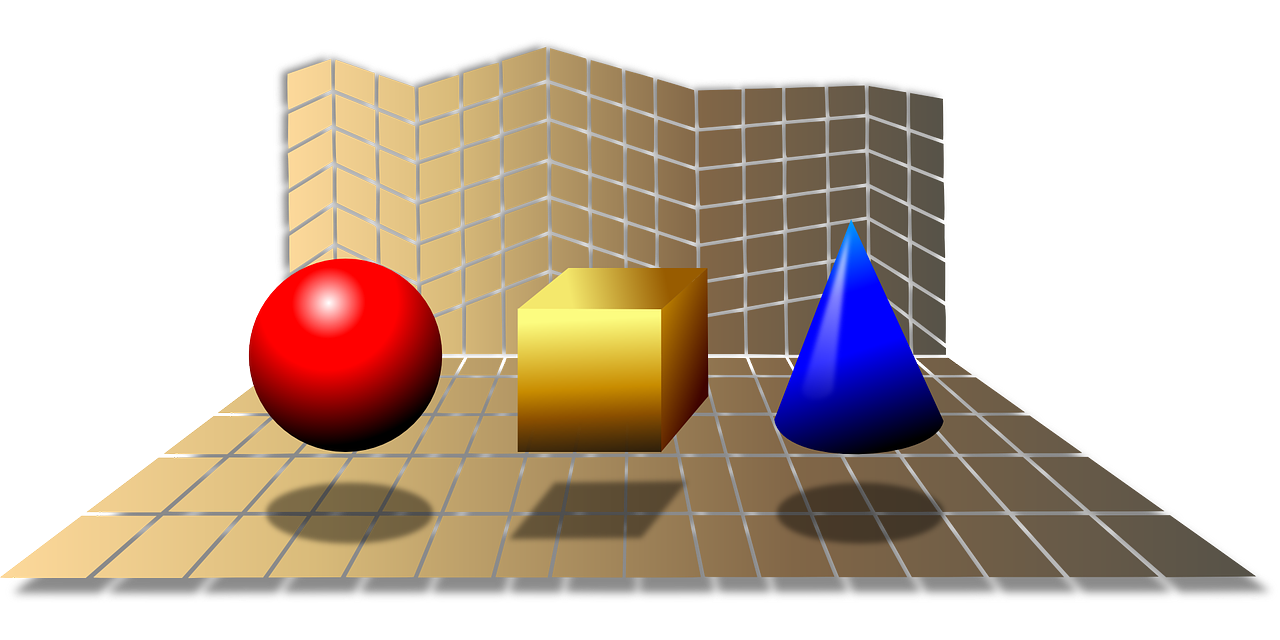
\includegraphics[width=1\textwidth]{imagenes/part4.png}}}

	
	
\chapter{Ideas básicas de la teoría de conjuntos} 
\chaptermark{Teoría de Conjuntos}\label{conjuntos}




\begin{tikzpicture}
	\fill [left color=teal!70, right color=gray!30] (0,0) rectangle (11.5,.1);
	\end{tikzpicture}
	


\begin{cita}{George \textsc{Cantor}}{Un conjunto es un “muchos” que puede ser pensado como uno.}\end{cita}

\section{Conjuntos}\label{cjtos}

\begin{definition}
	. Un \textbf{conjunto} es una colección de objetos con características similares considerada en sí misma como un objeto.
	
	Cada uno de los objetos que forman el conjunto recibe el nombre de \textbf{elemento} del conjunto.
\end{definition}

Un conjunto puede definirse por \emph{extensión} (nombrando a todos sus elementos) o por \emph{comprensión} (dando una propiedad que nos permita discernir si un objeto dado es o no un elemento del conjunto). Cuando el conjunto se define por extensión y ésta sea larga, se procede a definirlo \emph{por recurrencia} o mediante una expresión generalista.

Los conjuntos se designan por letras mayúsculas del alfabeto latino, $A,\ $ $B, \ $ $C,\ $ $\cdots$  Los elementos de un conjunto se dan entre llaves y se suelen representar por letras minúsculas del alfabeto latino, $\{a,\ b,\ c,\ \cdots \}$.

\begin{destacado}
	\emph{Nótese que en los conjuntos no es importante el orden en que se den sus elementos.}
\end{destacado}

\begin{definition}
	. El conjunto que no contiene ningún elemento se le llama \textbf{conjunto vacío} y se representa por el símbolo $\emptyset=\{\}$. 

	Este conjunto se define como una necesidad para cuadrar toda la teoría de conjuntos.
\end{definition}

\begin{definition}
. \textbf{Relación de pertenencia}  Se dice que un elemento $a$ \emph{pertenece} a un conjunto A si es de él, se representa así: $\ a\in A$. En caso contrario, se dice que no pertenece, $\ a \notin A$	
\end{definition}


\begin{example} 
. \textbf{Ejemplos}	
\begin{enumerate}[a) ]
\vspace{-3mm} \item Conjunto de los resultados que se obtienen al lanzar un dado: $\ A=\{1,2,3,4,5,6\};\ $ $\ 3\in A,\ 9\notin A$.
\vspace{-3mm} \item Conjunto de los números naturales: $\ \mathbb N=\{1,2,3,\cdots\};\ $ $\ 5\in \mathbb N,\ 2.47 \notin \mathbb N$.
\vspace{-3mm} \item El conjunto de los múltiplos naturales de $7$ es $\ \dot{7}=\{7,14,21,\cdots\}=\{7n,\ \forall n\in \mathbb N\};\ 91 \in \dot 7,\ 163 \notin \dot 7$.
\vspace{-3mm} \item Los números naturales, enteros, racionales, reales y complejos se designan, respectivamente, por las letras $\mathbb N,\ \mathbb Z,\ \mathbb Q,\ \mathbb R,\ \mathbb C$.
\vspace{-3mm} \item La expresión $\mathbb R\sim \{0,1\}$ indica en conjunto de todos los números reales a excepción del número $0$ y del $1$.
\end{enumerate}
\end{example}

\subsection{Subconjuntos}

\begin{definition}
	. Dado un conjunto $A$, a cualquier conjunto $B$ formado por cualquier número de elementos de $A$	se le llama  \textbf{subconjunto} de $A$.
	
	\vspace{2mm} Entre los posibles subconjuntos de $A$ están, obviamente, el conjunto vacío $\emptyset$ y el propio conjunto $A$. Estos subconjuntos reciben el nombre de `subconjuntos impropios'.

\end{definition}

Para indicar que $B$ es un subconjunto de $A$ se escribe $B \subset A$ y se lee ``$B$ está contenido o incluido en $A$''. Este símbolo se puede usar al revés, entones $A \supset B$ y se lee ``$A$ incluye o contiene a $B$''. Es un error escribir $B\in A$, el símbolo $\in$ se reserva solo para la pertenencia de elementos a conjuntos, pero si puede usarse tanto $a\in A$ como $\{a\}\subset A$. Al incluir un elemento entre llaves indicamos que se trata de un conjunto \emph{unitario}, formado por un único elemento. Si un conjuto $C$ no es subconjunto de $A$ se escribe $C \not\subset A$.

Es obvio que $\ \emptyset \subset A\ $ y que $\ A\subset A$. \textcolor{gris}{(En realidad, deberíamos escribir $A\subseteq A$).}

\begin{definition}
	. Se llama \textbf{cardinal} de un conjunto $A$, $\ card(A)\ $, al número de elementos que forman el conjunto $A$.
	
	Así, en el ejemplo anterior, $card(A)=6$; $card(\mathbb N)=\infty$, etc.
\end{definition}

\begin{definition}
	. Dado un conjunto $A$, el nuevo conjunto formado por todos los posibles subconjuntos de $A$ se llama conjuntos de las \textbf{partes} de $A$ y se representa por $\mathcal P(A)$.
	
	En 	$\mathcal P(A)$ se incluyen los subconjuntos `impropios' $\emptyset$ y el propio $A$.
\end{definition}



\begin{theorem}
	. Si un conjunto esta formado por $n$ elementos, el número de subconjuntos que se pueden formar a partir de $A$, incluyendo tanto el propio $A$ como al conjunto vacío $\emptyset$, es decir, el número de elementos de las partes de $A$ es $2^n$, es decir:
	
	$$\colorbox{orange!45}{ \boxed{ \  \boldsymbol{ \text{Si }\ card(A)=n \ \to \ card(\ \mathcal P(A)\ )	=2^n } \ } }$$
\end{theorem}



\begin{proof}
	\textcolor{gris}{La demostración de este teorema se hace usando combinatoria\footnote{ver apéndice \ref{combinatoria} `Combinatoria'}	y el binomio de Newton\footnote{\tiny{ Binomio de Newton:$(a+b)^n=\mqty(n\\0)a^nb^0+\mqty(n\\1)a^{n-1}b^1+\mqty(n\\2)a^{n-2}b^2+\cdots+\mqty(n\\n)a^0b^n$}}.}
	
	 \textcolor{gris}{Si el conjunto $A$ tiene $n$ elementos, el número de subconjuntos con $k$ elementos es igual al número combinatorio $C(n, k)= \mqty(n\\k) $. Un subconjunto de $A$ puede tener $0$ elementos como mínimo \textcolor{gris}{($\emptyset$)}, y $n$ como máximo \textcolor{gris}{($A$)}, y por lo tanto:}
	 
	 \textcolor{gris}{$$\boldsymbol{card(\ \mathcal P(A)\ )=^{_1}} \mqty(n\\0)+\mqty(n\\1)+\mqty(n\\2)+\cdots +\mqty(n\\n)=^{_2}(1+1)^n \boldsymbol{=2^n}$$ }
	 \rule{70mm}{0.1mm}
\end{proof}


\begin{example}
	. En el conjunto $D=$ resultados obtenidos al lanzar un dado `quinielístico', $X=\{1,X,2\}$, que tiene $3$ elementos, podemos considerar hasta $8=2^3$ subconjuntos posibles. Así:
	
	\begin{itemize}
	\vspace{-3mm}\item	Subconjuntos de cero elementos: $\ \{\}= \emptyset$
	\vspace{-3mm}\item	Subconjuntos de un elemento: $\ \{1\},\ \{X\}, \ \{2\}$ 
	\vspace{-3mm}\item	Subconjuntos de dos elementos: $\ \{1\,X\},\ \{X,2\}, \ \{1,2\} $
	\vspace{-3mm}\item 	Subconjuntos de tres elementos $\{1,X,2\}=Q$
	\end{itemize}
	
	Total, $8$ subconjuntos.
\end{example}


\begin{theorem}
	. La relación de inclusión cumple las siguientes propiedades:
	
	\begin{itemize}
	\vspace{-3mm} \item Si $C\subset B \ \wedge \ B \subset A \ \to \ C \subset A$
    \vspace{-3mm} \item Si $B \subset A \ \wedge \ A \subset B \ \to \ A=B$
	\vspace{-3mm} \item $\forall A \ , \ \ \emptyset \subset A$
	\end{itemize}
	
	\begin{scriptsize}
	\begin{quotation}
		\textcolor{gris}{ \emph{\underline{Nota:}}}
		
		\textcolor{gris}{El símbolo $\ \wedge \ $ equivale a la conjunción (lógica) \textbf{``y''}}. 
		
		\textcolor{gris}{El símbolo $\ \vee \ $ equivale a la disyunción (lógica) \textbf{``o''} .}
	\end{quotation}
	\end{scriptsize}
	
\end{theorem}

\begin{definition}
	. Si $B\subset A$, se llama \textbf{complementario} de $B$ respecto de $A$ al subconjunto de $A$ formado por todos los elementos que no estén en $B$.
	El complementario de un subconjunto se representa por uno de estos símbolos: $\ B',\ B^C,\ \overline{B};\  \neg B$	
	
	
	\small{El complementario siempre hace referencia a un `todo' o conjunto de referencia $E$, así, el complementario de $B$ será lo que le falta a $B$ para ser `todo', estará formado por todos los elementos (del conjunto referencial $E$) excepto los del propio $B$, esquemáticamente: $\ B'=E\sim B$, donde con $\sim$ queremos representar lo que acabamos de decir \textcolor{gris}{(coger todos los elementos de $E$ excepto -$\ \sim \ $- los de $B$)}}
	
	Obviamente, $\ \boxed{ \boldsymbol{ \ (A')'=A;\ \ E'=\emptyset; \ \ \emptyset'=E \ }}$
\end{definition}

\begin{example}

	. 	\begin{enumerate}[a) ]
	\item $E=\{1,2,3,4,5,6\}	 \ \wedge \ B=\{1,3\} \ \to \ B'=\{2,4,5,6\}$
	\item $\mathbb R^+=]0,+\infty[ \ \to \ (\mathbb R^+)'=]-\infty,0]=\mathbb R^- \text{ y el } 0$
	\item $[1,3]^C = \mathbb R \sim [1,3]$
	
	No confundir con  $ \ \mathbb R \sim [1,3] \ $ con $ \ \mathbb R \sim \{1,3\} \ $
	\end{enumerate}	
	
	\vspace{-5mm} %**********************************************
	\begin{figure}[H]
	\centering
	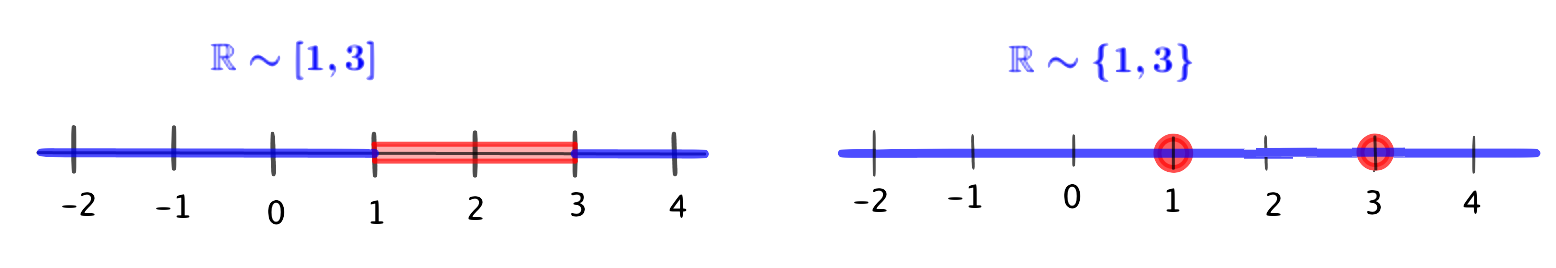
\includegraphics[width=.9\textwidth]{imagenes/apendices/app01.png}
	\end{figure}

\end{example}

\subsection{Diagramas de Venn}

\begin{multicols}{2}

	\begin{small}Los diagramas de Venn son esquemas usados en la teoría de conjuntos. Estos diagramas muestran `colecciones' (conjuntos) de `objetos' (elementos) por medio de líneas cerradas. La línea cerrada exterior abarca a todos los elementos bajo consideración, es el conjunto universal o referencial $E$.\end{small}
		
	\begin{figure}[H]
	\centering
	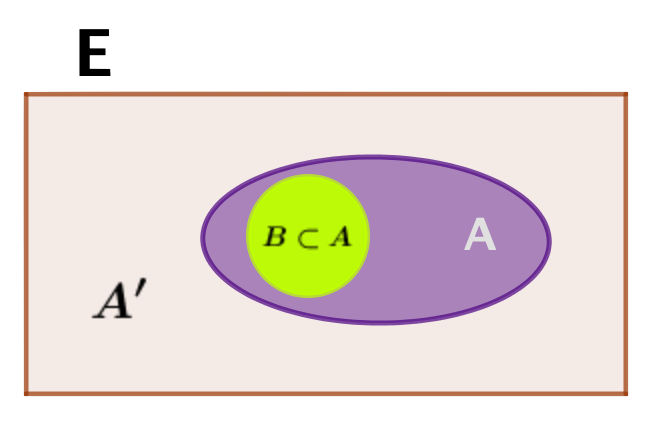
\includegraphics[width=.4\textwidth]{imagenes/apendices/app02.png}
	\end{figure}
	
\end{multicols}

Los diagramas de Venn fueron ideados hacia 1880 por John Venn.

\section{Operaciones con conjuntos}
\subsection{Unión e Intersección de conjuntos}

\begin{definition}
	. La \textbf{unión} de dos conjuntos $A \text{ y } B$	, que se denota por $\ \boldsymbol{A\cup B}\ $, es el conjunto formado por todos los elementos que pertenecen a $A$ o a $B$, los elementos que pertenecen a cualquiera de los dos conjuntos.
	
	\vspace{3mm} La \textbf{intersección} de dos conjuntos $A \text{ y } B$	, que se denota por $\ \boldsymbol{A\cap B}\ $, es el conjunto formado por todos los elementos que pertenecen a $A$ y a $B$ simultáneamente, es decir, los elementos comunes a $A$ y a $B$.
	
	\begin{multicols}{2}
	\begin{figure}[H]
	\centering
	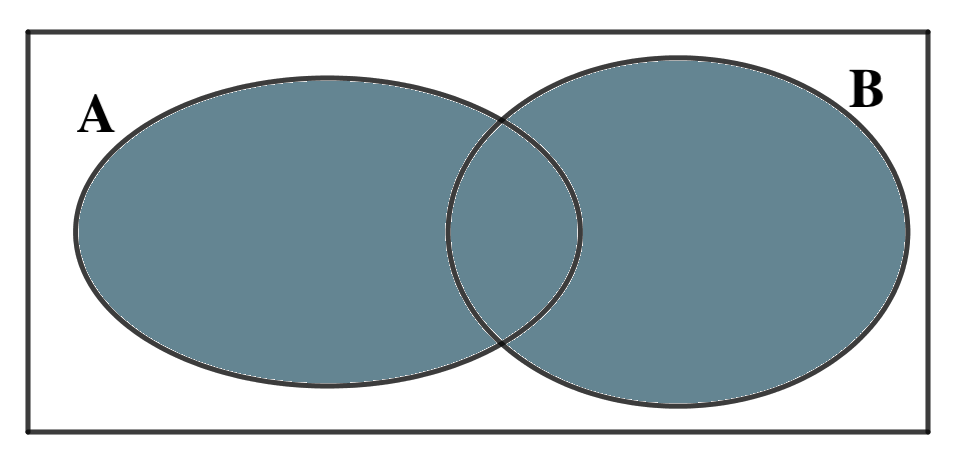
\includegraphics[width=.45\textwidth]{imagenes/apendices/app03.png}
	\caption*{$A\cup B$}
	\end{figure}
	\vspace{-13mm}
	$$A\cup B=\{x/\ x\in A \ \vee \ x \in B\}$$
	\begin{figure}[H]
	\centering
	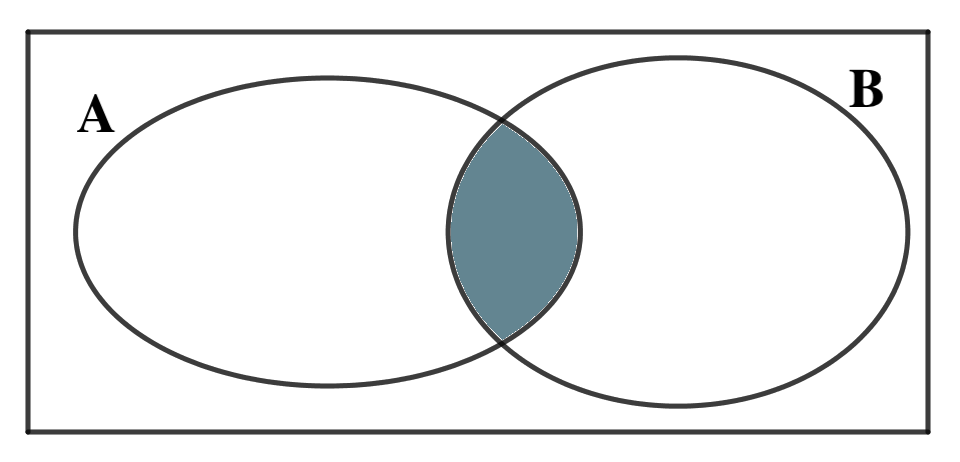
\includegraphics[width=.45\textwidth]{imagenes/apendices/app04.png}
	\caption*{$A\cap B$}
	\end{figure}
	\vspace{-13mm}
	$$A\cap B=\{x/\ x\in A \ \wedge \ x \in B\}$$
	\end{multicols}
\end{definition}

\begin{myexampleblock}{Chiste}
	\begin{figure}[H]
	\centering
	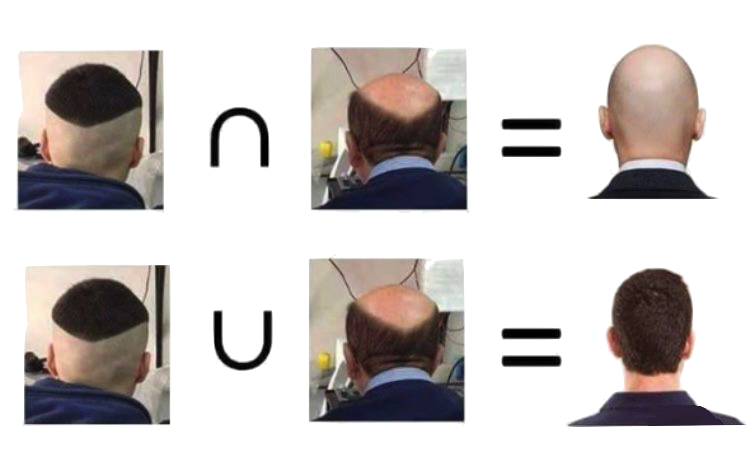
\includegraphics[width=.9\textwidth]{imagenes/apendices/app10b.png}
	\end{figure}
\end{myexampleblock}

\begin{theorem}
	. Propiedades de la unión e intersección de conjuntos.
		
		\begin{multicols}{2}
		\begin{itemize}
		\vspace{-3mm} \item $A\cup B=B\cup A$
		\vspace{-3mm} \item $A\cup \emptyset=A$
		\vspace{-3mm} \item $A\cup E=E$
		\vspace{-3mm} \item $A\cup A'=E$
		\end{itemize}
		\begin{itemize}
		\vspace{-3mm} \item $A\cap B=B\cap A$
		\vspace{-3mm} \item $A\cap \emptyset=\emptyset$
		\vspace{-3mm} \item $A\cap E=A$
		\vspace{-3mm} \item $A\cap A'=\emptyset$
		\end{itemize}
		\end{multicols}

\end{theorem}

\begin{definition}
	. Si $\ A\cap B=\emptyset \ \to \ $ se dice que $A\text{ y } B$ son \textbf{disjuntos}	
\end{definition}

\begin{example}
	.  \begin{enumerate}[a) ]

	\item Sean $A=\{a,A,e\};\ B=\{A,B\} \ \to $
	
	$\qquad \ A\cup B=\{a,e,A,B\}; \ A\cap B=\{A\}$.
	
	\item Sean $\dot 3=\{3,6,9,12, \cdots\}; \ \dot 5=\{5,10,15,\cdots \} \ \to$
	
	$\qquad \ A\cup B=\{3,5,6,9,10, \cdots \}; \ A\cap B=\{15,30,\cdots\}$ \textcolor{gris}{(mcm)}.
	
\end{enumerate}
\end{example}

\begin{theorem}
	. $$\subrayado{\boxed{\ \boldsymbol{  card(A\cup B)= card (A) + card B - card(A\cap B) } \ }	}$$
\end{theorem}


\begin{figure}[H]
	\centering
	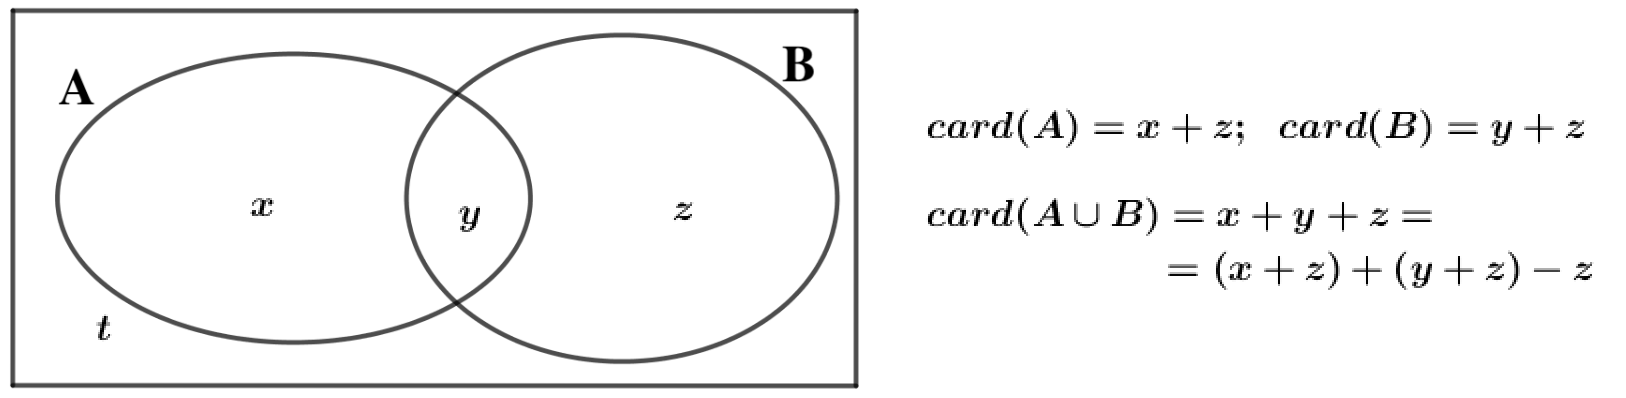
\includegraphics[width=.8\textwidth]{imagenes/apendices/app13.png}
	\end{figure}


\begin{example}
	. \begin{small}
	Se sabe que, de los 100 alumnos de bachillerato (conjunto referencial), a 30 les gusta la Anatomía (cardinal del conjuto A), a 40 la Biología (cardinal del conjunto B) y a 10 les gustan ambas asignaturas (cardinal de la intersección).	 ?`A cuántos alumnos les gustan alguna de estas asignaturas ($card(A\cup B$)? ?`A cuántos de ellos no les gusta ninguna ($card(AUB)'$)? 
	
	El siguiente diagrama ilustra la solución y da un ejemplo que aclara el teorema anterior.

	\begin{figure}[H]
	\centering
	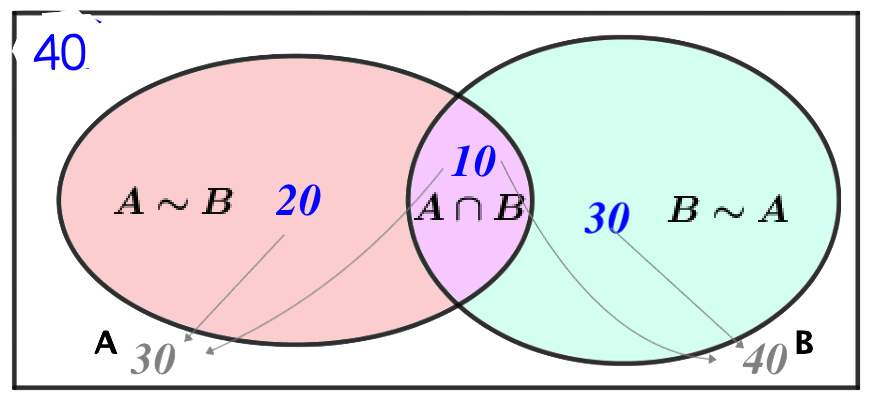
\includegraphics[width=.6\textwidth]{imagenes/apendices/app07.png}
	\end{figure}
	
	De los 30 alumnos que les gusta Anatonía, a 10 de ellos también les gusta la biología (pues les gustan las dos asignaturas); quedan 30-10=20 alumnos a los que solo les gusta la Anatomía. Un razonamiento análogo nos llevará a concluir que son 40-10=30 los alumnos a los que les gusta solo la biología. En total tendremos 20 alumnos que les gusta solo A, 30 que les gusta solo B y 10 que les gustan ambas, total 60 alumnos de los 100 a los que les gusta alguna de estas dos asignaturas. Hay, pues, 40 a los que no les gustan ninguna de ellas. 
	
	$card(A\cup B)=60;\quad card((A\cup B)')=40$
	\end{small}
\end{example}




\subsection{Diferencia de conjuntos}

\begin{definition}
	. Dados dos conjuntos $A \text{ y } B$, se llama conjunto \textbf{diferencia}, y se representa por $A\sim B$, al conjunto formado por todos los elementos de $A$ excluidos los que pertenecen a $B$.
	
	\vspace{-4mm} $$A\sim B=\{x/\ x\in A \ \wedge x \ \notin B\}	$$
	
	Análogamente: $\ B\sim A=\{x/\ x\in B \ \wedge x \ \ \notin A\}$
	
	\vspace{2mm} Obviamente $A\sim B \ \neq	\ B\sim A$
\end{definition}

\begin{theorem}
	. \vspace{-5mm} 
	
	\begin{small}
	$$\boxed{\boldsymbol{ A\sim B=A\cap B'}}\ ; \ \ \ \boxed{\boldsymbol{A\cup B=(A\sim B) \ \cup \ (A\cap B) \ \cup \ (B\sim A)}}$$ \end{small}
\end{theorem}

\begin{proof}

\begin{multicols}{2}
	\begin{figure}[H]
	\centering
	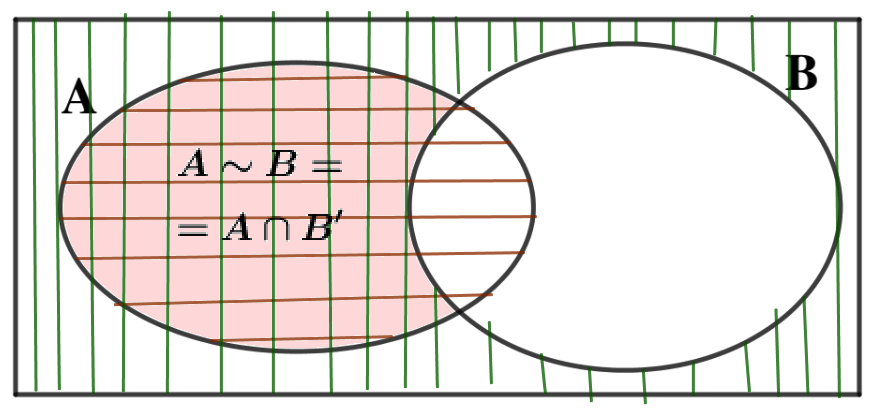
\includegraphics[width=.45\textwidth]{imagenes/apendices/app05.png}
	\end{figure}
	\begin{figure}[H]
	\centering
	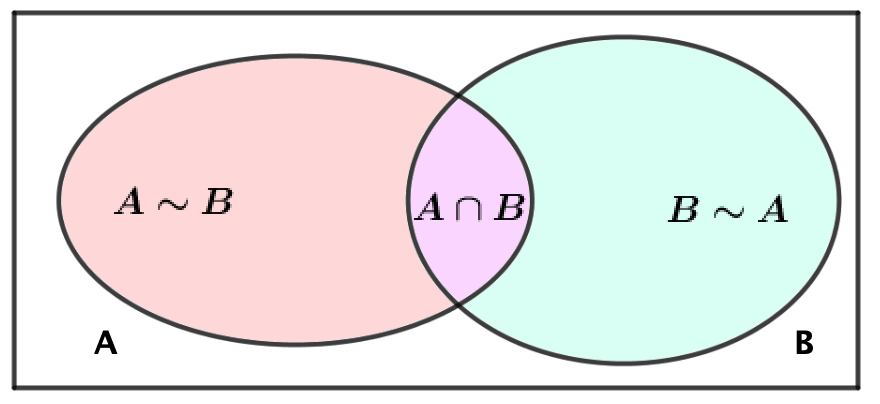
\includegraphics[width=.45\textwidth]{imagenes/apendices/app06.png}
	\end{figure}
\end{multicols}	

En la primera figura, hemos dibujado el conjunto $A$ con líneas horizontales y el $B'$ (todo lo que no es $B$), con líneas verticales. La intersección es la sección común en que se cruzan las líneas. (La unión sería todo lo que esté rayado de cualquier forma, vertical, horizontal o cruzado).

En la segunda figura, hemos dibujado en rojo el conjunto $A\sim B$, en azul el $B\sim A$ y en morado en $A\cap B$. La unión $A\cup B$ está formada por todas las secciones coloreadas. \textcolor{gris}{Los tres conjuntos son disjuntos entres sí.}
\end{proof}

\subsection{Producto cartesiano de dos conjuntos}

\begin{definition}
	. El producto cartesiano de dos conjuntos $A \text{ y } B$, que denotamos por $A\times B$, es el conjunto formado por todos los pares ordenados de elementos de $A$ y $B$ (el primer elemento del par ha de ser de $A$ y el segundo de $B$).
	
	\vspace{-4mm} $$A\times B= \{(a,b) \ / \ a\in A \ \wedge \ b\in B \}$$	
\end{definition}

\begin{example}
	. \begin{enumerate}[a) ]
 		\item $A=\{1,2,3\};\ B=\{a,b\} \ \to $
 		
 		$A\times B = \{(1,a),(1,b),(2,a),(2,b),(3,a),(3,b)\}$
 		
 		\item $\mathbb R \times \mathbb R=\mathbb R^2$ es el conjunto de los puntos del plano. $\mathbb R^3$ representa al espacio tridimensional, $\mathbb R^n$ un espacio de $n$ dimensiones.
 	\end{enumerate}
\end{example}

\section[Propiedades combinadas de las operaciones con conjuntos]{Propiedades combinadas de las operaciones con conjuntos\sectionmark{Propiedades}}
\sectionmark{Propiedades}

\begin{theorem}
	. \begin{itemize}
		\item Asociativas:
		
		\vspace{-5mm} $$A\cup(B\cup C)=(A\cup B)\cup C \qquad A\cap(B\cap C)=(A\cap B)\cap C$$
		
		\item Distributivas:
		
		\vspace{-5mm} $$A\cup(B\cap C)=(A\cup B)\cap (A\cup C) \qquad A\cap(B\cup C)=(A\cap B)\cup (A\cap C)$$
		
		\item \textbf{Leyes de Morgan}
		
		\vspace{-7mm} \begin{multicols}{2}

		\vspace{-5mm} $$\boldsymbol{ (A\cup B)'=A'\cap B'}$$
		
		``El complementario de la unión es la intersección de complementarios''.
		
		 \vspace{-5mm} $$\boldsymbol{ (A\cap B)'=A'\cup B' }$$
		
		``El complementario de la intersección es la unión de complementarios''.
	\end{multicols}	
		
   	\end{itemize}	
\end{theorem}

\begin{proof}.

	Mediante diagramas de Venn, es fácil demostrar estos teoremas.	
	
	\begin{figure}[H]
	\centering
	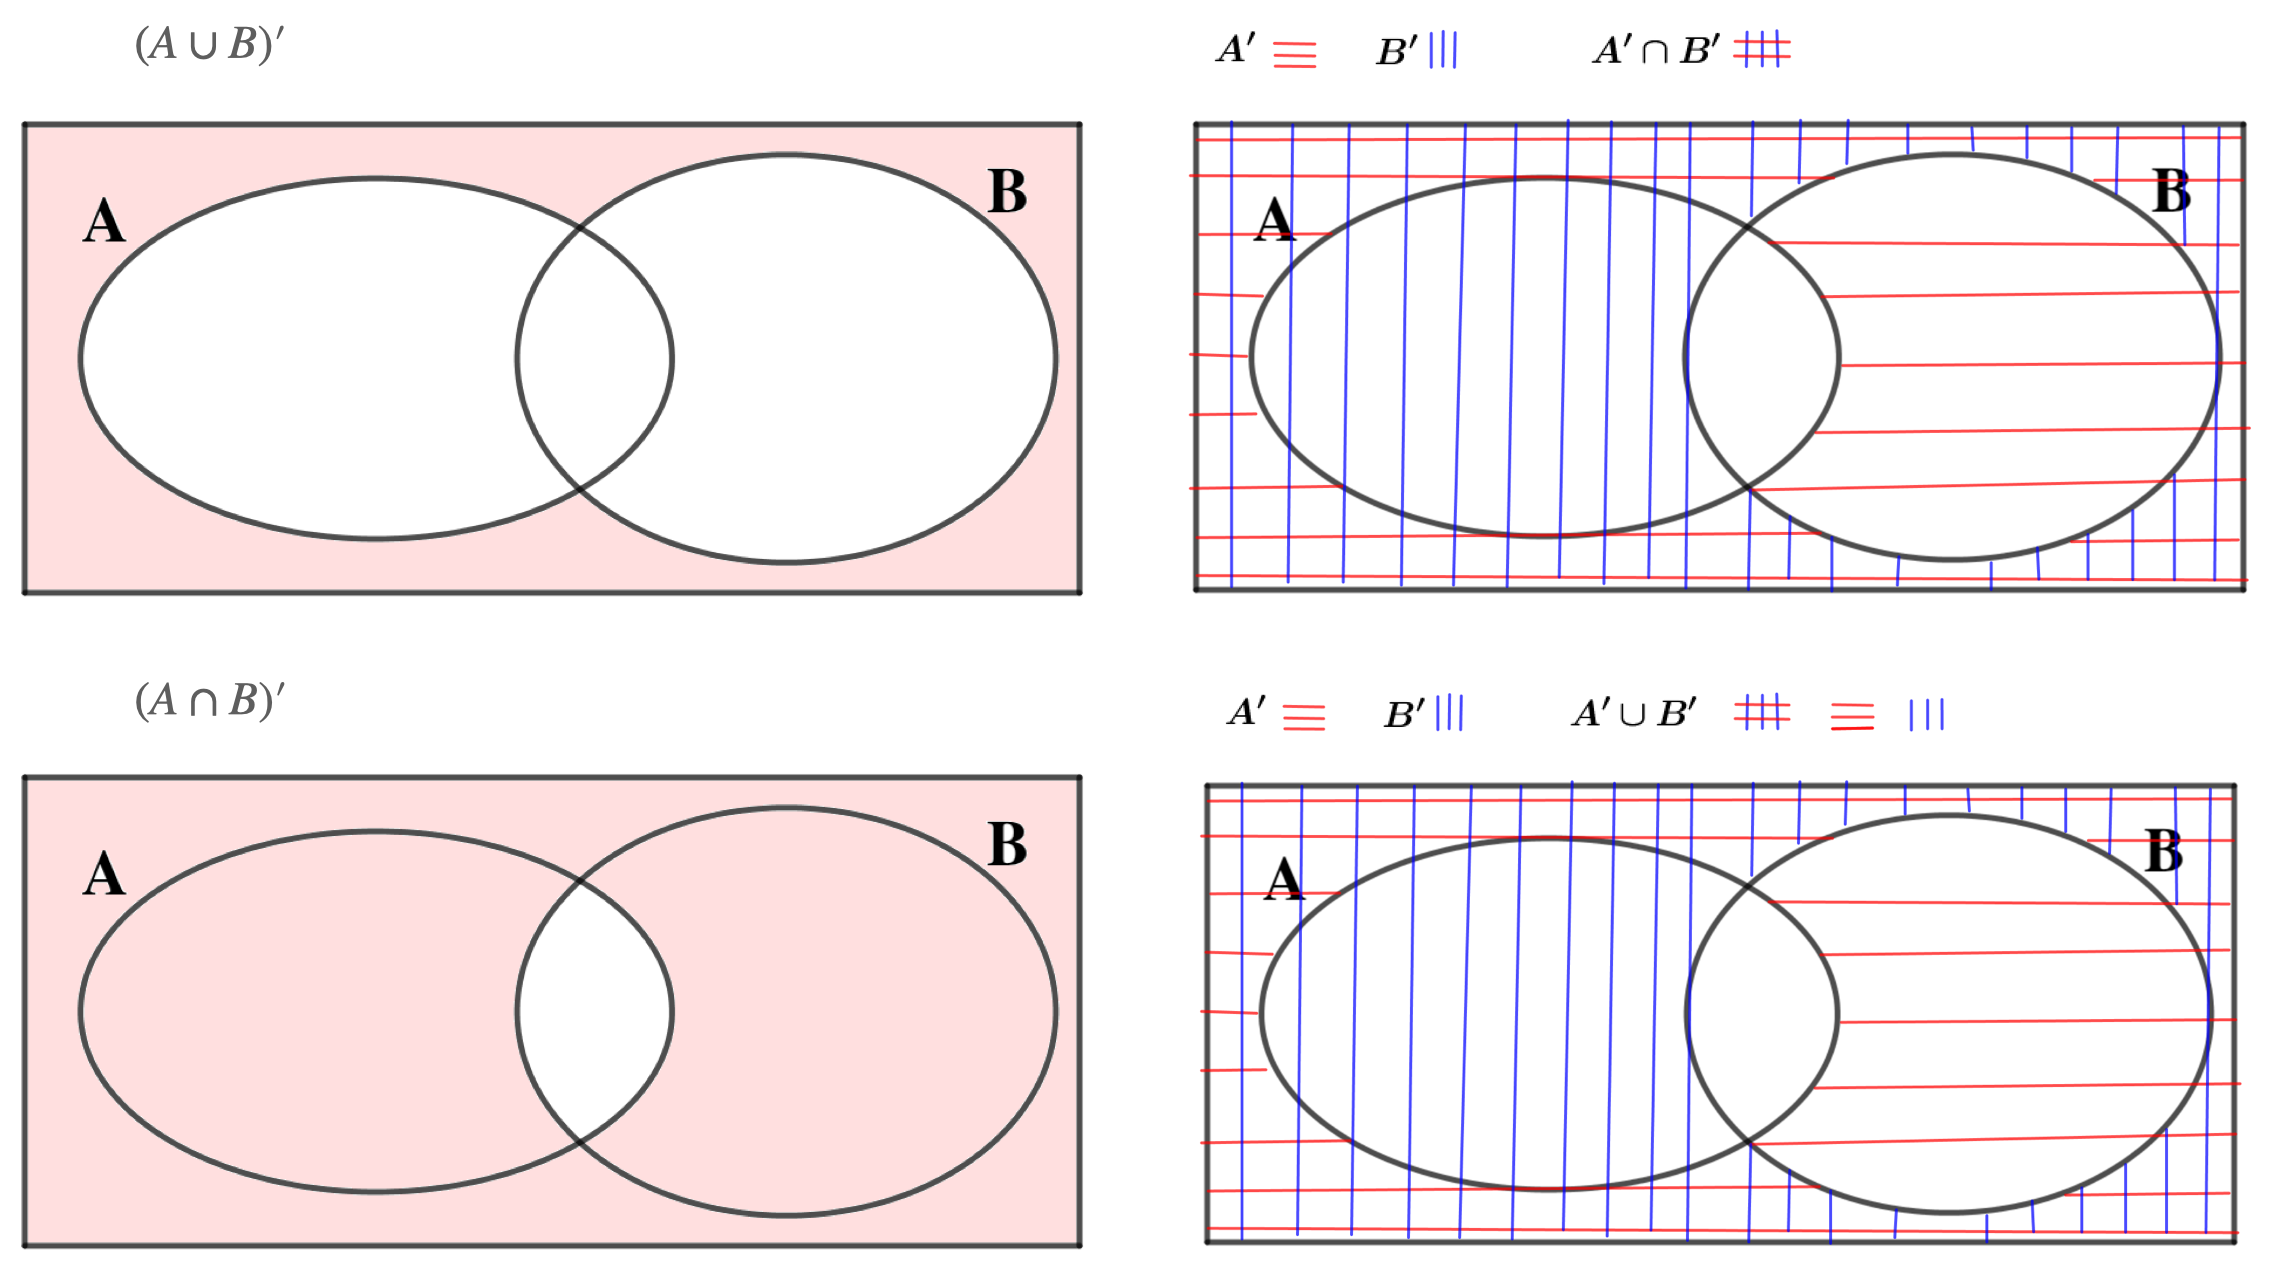
\includegraphics[width=.85\textwidth]{imagenes/apendices/app08.png}
	\caption*{Leyes de Morgan y diagramas de Venn.}
	\end{figure}
	
\end{proof}

\begin{example}
	. Si $M$ representa el conjunto de los habitantes de Madrid y $C$ el conjunto de los nacidos en Cataluña, entonces: 

\begin{itemize}
	\vspace{-2mm} \item $M\cup C$  representa el conjunto de las personas que viven en Madrid o que han nacido en Cataluña. 

	\vspace{-2mm} \item $(M\cup C)'$ representa a las personas que no viven en Madrid y que no han nacido en Cataluña. 

	\vspace{-2mm} \item $M'$ son las personas que no viven Madrid, y $C'$ aquellos que no han nacido en Cataluña. 

	\vspace{-2mm} \item $M'\cap C'$ serán las personas que no viven en Madrid y que tampoco han nacido en Cataluña.  Es evidente que $(M\cup C)'=M'\cap C'$. 

	\vspace{-2mm} \item Igualmente: $M\cap C$ representa el conjunto de las personas que viven en Madrid y que han nacido en Cataluña. 

	\vspace{-2mm} \item $(M\cap C)'$ representa a las personas que o no viven en Madrid o no han nacido en Cataluña. 

	\vspace{-2mm} \item $M'$ son las personas que no viven Madrid, y $C'$  aquellos que no han nacido en Cataluña. 

	\vspace{-2mm} \item  $M'\cup C'$ serán las personas que no viven en Madrid o que no han nacido en Cataluña.  Es evidente que $(M\cap C)'=M'\cup C'$. 
\end{itemize}

\end{example}

\begin{ejemplo}
\begin{ejre}
En una ciudad se editan tres revistas A, B y C. Se ha preguntado a un grupo de personas sobre la lectura o no de esos periódicos, obteniéndose los siguientes resultados:
\begin{itemize}
	\vspace{-2mm} \item Lectores de A: 32; lectores de B: 45; lectores de C: 23.
	\vspace{-2mm} \item Leen A y B 14 personas, A y C 9 y B y C 12.
	\vspace{-2mm} \item Leen las tres periódicos 5 personas.
	\vspace{-2mm} \item No leen ninguna revista 54 personas.	
\end{itemize}
?`A cuántas personas se les ha pasado la encuesta?.
\end{ejre}
\end{ejemplo}
	
	\begin{figure}[H]
	\centering
	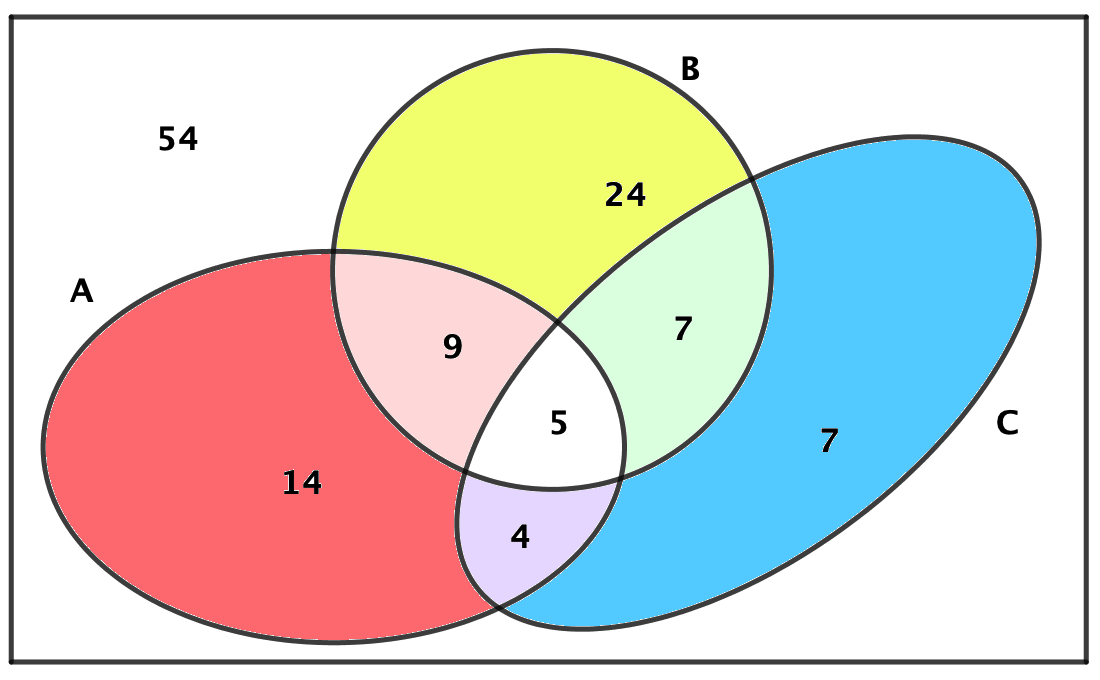
\includegraphics[width=.6\textwidth]{imagenes/apendices/app09.png}
	\end{figure}

\vspace{-5mm} $$54+14+9+24+4+5+7+7=124 \text{ personas encuestadas}$$




\chapter{Combinatoria. Técnicas de recuento} 
\chaptermark{Combinatoria}\label{combinatoria}


\vspace{-10mm}

\begin{tikzpicture}
	\fill [left color=teal!70, right color=gray!30] (0,0) rectangle (11.5,.1);
	\end{tikzpicture}
	


\begin{quotation}
	\emph{La combinaroria es la parte de las matemáticas que se ocupan de la resolución de problemas de elección y disposición de los elementos de un conjunto, atendiendo a ciertas reglas.}	
\end{quotation}

\section{Principio de multiplicación}

\begin{definition}
	. Si un principio de selección se puede separar en $\boldsymbol{r}$ etapas, de modo que el resultado de cada una de ellas no influya en la siguiente, y en cada uno de estas etapas se obtienen respectivamente $\ \boldsymbol{n_1,n_2,\cdots ,n_r}$ resultados, entonces el procedimiento global tiene $\ \displaystyle \boldsymbol{\prod_{i=1}^r n_i= n_1 \cdot n_2  \cdots  n_r}\ $ resultados.
\end{definition}

Veamos algunos ejemplos en los que nos ayudamos con un \textbf{\emph{diagrama de árbol}}:

\begin{example}
	. Distintos resultados en el lanzamiento de una monedas tres veces.
\vspace{4mm}
% Set the overall layout of the tree
\tikzstyle{level 1}=[level distance=1.5cm, sibling distance=2cm]
\tikzstyle{level 2}=[level distance=1.5cm, sibling distance=1cm]
\tikzstyle{level 3}=[level distance=3cm, sibling distance=.5cm]

% Define styles for bags and leafs
\tikzstyle{bag} = [text width=2em, text centered]
\tikzstyle{end} = [circle, minimum width=3pt,fill, inner sep=0pt]

\begin{tikzpicture}[grow=right, sloped]
\node {}
    child {
        node[bag] {$X$}  
            child {
                node {$X$}{}
            		child {
            		node {$X \qquad \textcolor{gris}{XXX}$}
            		}
            		child {
            		node {$C  \qquad \textcolor{gris}{XXC} $}
            		}
            }
            child {
                node {$C$}{}
            		child {
            		node {$X  \qquad \textcolor{gris}{XCC} $}
            		}
            		child {
            		node {$C  \qquad \textcolor{gris}{XCX} $}
            		}
            }
    }
    child {
        node[bag] {$C$}   
            child {
                node {$X$} {}
                	child {
            		node {$X  \qquad \textcolor{gris}{CXC} $}
            		}
            		child {
            		node {$C  \qquad \textcolor{gris}{CXX} $ }
            		}
            }
            child {
                node {$C$} {}
               		child {
            		node {$X  \qquad \textcolor{gris}{CCX} $}
            		}
            		child {
            		node {$C  \qquad \textcolor{gris}{CCC} $}
            		}
            } 
    }
    ;
\end{tikzpicture}
$$2\cdot 2\cdot 2 = 8 \text{ posibilidades}$$
\end{example}

\begin{example}
	. En un restaurante el menú se pueden elegir
entre dos primeros platos (P) , tres segundos (S) y
dos postres (Po). ?`Cuántos menús diferentes
se pueden pedir?	

\vspace{4mm}
% Set the overall layout of the tree
\tikzstyle{level 1}=[level distance=1.5cm, sibling distance=3cm]
\tikzstyle{level 2}=[level distance=1.5cm, sibling distance=1cm]
\tikzstyle{level 3}=[level distance=1.5cm, sibling distance=.5cm]

% Define styles for bags and leafs
\tikzstyle{bag} = [text width=2em, text centered]
\tikzstyle{end} = [circle, minimum width=3pt,fill, inner sep=0pt]

\begin{tikzpicture}[grow=right, sloped]
\node {}
    child {
        node[bag] {$P2$}  
            child {
                node {$S3$}{}
            		child {
            		node[end, label=right: {$Po2 \textcolor{gris}{\qquad \text{menú: }P2S3Po2}\quad 12\text{ menús}$}] {}
            		}
            		child {
            		node[end, label=right: {$Po1 \textcolor{gris}{\qquad \text{menú: }P2S3Po1}$}] {}
            		}
            }
            child {
                node {$S2$}{}
            		child {
            		node[end, label=right: {$Po2 \textcolor{gris}{\qquad \text{menú: }P2S2Po2}$}] {}
            		}
            		child {
            		node[end, label=right: {$Po1 \textcolor{gris}{\qquad \text{menú: }P2S2Po1}$}] {}
            		}
            }
            child {
                node {$S1$}{}
            		child {
            		node[end, label=right: {$Po2 \textcolor{gris}{\qquad \text{menú: }P2S1Po2}$}] {}
            		}
            		child {
            		node[end, label=right: {$Po1 \textcolor{gris}{\qquad \text{menú: }P2S1Po1}$}] {}
            		}
            }
    }
    child {
        node[bag] {$P1$}   
            child {
                node {$S3$} {}
            		child {
            		node[end, label=right: {$Po2 \textcolor{gris}{\qquad \text{menú: }P1S3Po2}$}] {}
            		}
            		child {
            		node[end, label=right: {$Po1 \textcolor{gris}{\qquad \text{menú: }P1S3Po1}$}] {}
            		}
            }
            child {
                node {$S2$} {}
                	child {
            		node[end, label=right: {$Po2 \textcolor{gris}{\qquad \text{menú: }P1S2Po2}$}] {}
            		}
            		child {
            		node[end, label=right: {$Po1 \textcolor{gris}{\qquad \text{menú: }P1S2Po1}$}] {}
            		}
            }
            child {
                node {$S1$} {}
               		child {
            		node[end, label=right: {$Po2 \textcolor{gris}{\qquad \text{menú: }P1S1Po2}$}] {}
            		}
            		child {
            		node[end, label=right: {$Po1 \textcolor{gris}{\qquad \text{menú: }P1S1Po1}$}] {}
            		}
            } 
    }
    ;
\end{tikzpicture}
$$2\cdot 3\cdot 2 = 12 \text{ posibilidades}$$
\end{example}

\begin{myexampleblock} {El principio del palomar}
\begin{small}
También llamado principio de Dirichlet o principio de las cajas, establece que si $n$ palomas se distribuyen en $m$ palomares, y si $n > m$, entonces al menos habrá un palomar con más de una paloma. A manera de ejemplo: si se toman trece personas, al menos dos habrán nacido el mismo mes.

\vspace{2mm} Aunque el principio del palomar puede parecer una observación trivial, se puede utilizar para demostrar resultados inesperados. Por ejemplo, hay por lo menos 2 personas en Guatemala con el mismo número de pelos en la cabeza. 
\end{small}
\begin{multicols}{2}
\begin{small}
	\underline{Demostración}: la cabeza de una persona tiene en torno a 150.000 cabellos y tener un millón de pelos requeriría de una cabeza gigante (nadie tiene un millón de pelos en la cabeza). Asignamos un palomar por cada número de 0 a 1.000.000 y asignamos una paloma a cada persona que irá al palomar correspondiente al número de pelos que tiene en la cabeza. Como en Guatemala hay más de un millón de personas, habrá al menos dos personas con el mismo número de pelos en la cabeza. 
\begin{figure}[H]
	\centering
	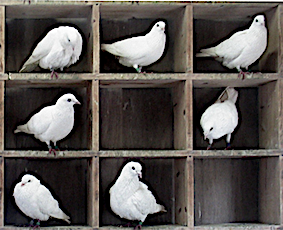
\includegraphics[width=.45\textwidth]{imagenes/apendices/app14.png}
	\end{figure}
\end{small}
\end{multicols}
\begin{flushright}\begin{scriptsize}\textcolor{gris}{Wikipedia}\end{scriptsize}\end{flushright}
\end{myexampleblock}



\section{Permutaciones}

\begin{definition}
	. Se llama \textbf{factorial} de un número natural $n\in \mathbb N$ y se denota como $ \ \boldsymbol{n!} \ $	:
	$ \quad \ \boxed{ \ \boldsymbol{ n!=n \cdot (n-1) \cdot (n-2) \cdots \cdot 3 \cdot 2 \cdot 1 } \ } $
	
	\vspace{2mm} Por convenio, se define $\ \boldsymbol{0!=1}$
\end{definition}

\begin{definition}
	. Se llama \textbf{permutaciones de $n$ elementos}, $P_n$,  todos ellos distintos, al número de ordenaciones de 	esos elementos.
	
	$$ \boxed{\ \boldsymbol{P_n \ = \ n! }  \ } \textcolor{gris}{\ =n \cdot (n-1) \cdot (n-2) \cdots \cdot 3 \cdot 2 \cdot 1 } $$
\end{definition}

\begin{small}
Esto es obvio. De los $n$ elementos a ordenar, el primero lo poedemos elegir de $n$ formas distintas. Por cada una de ellas quedan $n-1$ elementos de los que podemos escoger el segundo a ordenar de $n-1$ formas distintas. Para el tercer elemento, hay $2$ escogidos y quedan $n-2$ por escoger, lo podemos hacer de $n-2$ formas distintas; etc. Cuando queden solo dos elementos, ya hay $n-2$ elegidos, tenemos $2$ formas distintas de hacerlo; para cada una de estas elecciones quedará solo $1$ elemento a escoger que podremos hacer de $1$ sola forma. Usando el principio de multiplicación, tendremos:
$\quad P_n   =n \cdot (n-1) \cdot (n-2) \cdots \cdot 3 \cdot 2 \cdot 1 $. 
\end{small}

\begin{example}
	. ?`Cuántos números distintos, de tres cifras y ninguna de ellas repetidas, podemos obtener con los dígitos $ \{ 3,5,7 \} $	
	
	\vspace{3mm} Se trata de obtener todas las ordenaciones posibles de tres elementos, por tanto, la solución es $P_3=3!=6$ números distintos.
	
	Ilustramos estos números con un diagrama de árbol.
	
	\vspace{4mm}
% Set the overall layout of the tree
\tikzstyle{level 1}=[level distance=2.5cm, sibling distance=1cm]
\tikzstyle{level 2}=[level distance=1.5cm, sibling distance=.5cm]
\tikzstyle{level 3}=[level distance=1.5cm, sibling distance=0cm]

% Define styles for bags and leafs
\tikzstyle{bag} = [text width=2em, text centered]
\tikzstyle{end} = [circle, minimum width=3pt,fill, inner sep=0pt]


\begin{center}
\begin{tikzpicture}[grow=right, sloped]
\node {}
	child {
        node[bag] {$3$}  
            child {
                node {$2$}{}
            		child {
            		node {$1 \qquad \textcolor{gris}{321}$}
            		}
            }
            child {
                node {$1$}{}
            		child {
            		node {$2  \qquad \textcolor{gris}{312} $}
            		}
            }
    }
    child {
        node[bag] {$2$}  
            child {
                node {$3$}{}
            		child {
            		node {$1 \qquad \textcolor{gris}{231}$}
            		}
            }
            child {
                node {$1$}{}
            		child {
            		node {$3  \qquad \textcolor{gris}{213} $}
            		}
            }
    }
    child {
        node[bag] {$1$}   
            child {
                node {$3$} {}
                	child {
            		node {$2  \qquad \textcolor{gris}{132} $}
            		}
            }
            child {
                node {$2$} {}
               		child {
            		node {$3  \qquad \textcolor{gris}{123} $}
            		}
            } 
    }
    ;
\end{tikzpicture}
\end{center}
\end{example}

\begin{small}
	\textcolor{gris}{El primer dígito del número puede ser de los tres dígitos; elegido éste, el segundo puede ser cualquiera de los dos que quedan y ya solo quedaría una posibilidad para el tercer dígito. Por el principio de superposición, $3\cdot 2 \cdot 1 1=6$ números distintos.}	
	\end{small}

\begin{example}
	. ?`De cuantas maneras distintas se pueden colocar $10$ libros distintos en el balde de una estantería?
	
	\vspace{4mm} El primer libro, de derecha a izquierda, por ejemplo, puede ser cualquiera de los $10$; el segundo, cualquiera de los $9$ restantes, ...
	
	\vspace{2mm} $P_{10}=10!=3628800$ formas de ordenación distintas.	
\end{example}


\subsection{Permutaciones con repetición}

\begin{definition}
	. Para calcular el número de ordenaciones posibles de $n$ elementos de los cuales hay $n_1$ repetidos, $n_2$ repetidos, etc; de modo que $n_1+n_2+\cdots +n_r=n$ se usan las \textbf{permutaciones con repetición}.
	
	$$ \boxed{ \ \boldsymbol{ PR_n^{n_1,n_2,\cdots ,n_r} \ = \ \dfrac{n!}{n_1!\cdot n_2! \cdots n_r!} } \ } $$	
\end{definition}

\begin{example}
	. ?`De cuantas maneras distintas se pueden colocar $10$ libros  en el balde de una estantería, si hay $5$ de ellos iguales entre sí y también $3$ de ellos iguales?
	
	\vspace{4mm} Se trata de ordenar $10$ objetos de los cuales hay $5,3,1,1$ repetidos \textcolor{gris}{$(5+3+1+1=10)$.}
	
	\vspace{2mm} $PR_{10}^{5,3,1,1}=\dfrac{10!}{5! \cdot 3!}= \small{\dfrac{10\cdot 9 \cdot 8 \cdot 7 \cdot \bcancel{6} \cancel{\cdot 5 \cdot 4 \cdots 1}}{\cancel{5\cdot 4\cdots 1} \ \cdot \ \bcancel{3\cdot 2}}}=5040$ \normalsize{ordenaciones.}	
\end{example}

\begin{example}
	. Con los dígitos $1,1,1,2,2,3$, ?`cuántos números distintos con las  seis cifras pueden formarse	?
	
	\vspace{4mm} $PR_6^{3,2,1}=\dfrac{6!}{3!\cdot 2!}=60$ números distintos.
\end{example}

\begin{small}
Si los dígitos fuesen distintos, $\textcolor{red}{1}, \textcolor{green}{1}, \textcolor{blue}{1}, \textcolor{violet}{2}, \textcolor{teal}{2}, 3$, tendríamos un total de $6!$ ordenaciones distintas.

Pero, ocurre que las ordenaciones  $\textcolor{red}{1}, \textcolor{green}{1}, \textcolor{blue}{1}, \textcolor{violet}{2}, \textcolor{teal}{2}, 3$ y  $\textcolor{green}{1}, \textcolor{red}{1}, \textcolor{blue}{1}, \textcolor{violet}{2}, \textcolor{teal}{2}, 3$ (se ha alterado el orden de los unos) son el mismo número, y así hay $3!$ posibilidades distintas, por lo que al resultado anterior $6!$, hay que dividirlo entre estas $3!$ ordenaciones que conducen al mismo número. 

Lo mismo para el dígito $2$, hay $2!$ formas inicialmente distintas que conducen al mismo número,  $\textcolor{red}{1}, \textcolor{green}{1}, \textcolor{blue}{1}, \textcolor{violet}{2}, \textcolor{teal}{2}, 3$ y  $\textcolor{red}{1}, \textcolor{green}{1}, \textcolor{blue}{1}, \textcolor{teal}{2}, \textcolor{violet}{2}, 3$, por lo que hay que dividir el resultado anterior $6!/3!$ entre $2!$ obteniéndose el resultado final $6!/(3!\cdot 2!)=PR_6^{3,2}\textcolor{gris}{(=PR_6^{3,2,1})}$.
\end{small}

\subsection{Permutaciones circulares}

\begin{definition}
	. Las \textbf{permutaciones circulares} son un caso particular de las permutaciones.

\vspace{2mm} Se utilizan cuando los elementos se han de ordenar ``en círculo'', (por ejemplo, los comensales en una mesa), de modo que el primer elemento que ``se sitúe'' en la mesa determina el principio y el final de muestra, quedando tan solo $n-1$ elementos que ordenar:	
 
 $$ PC_n=(n-1)!$$
\end{definition}

\begin{small} Al ordenar $n$ elementos en una posición circular, la posición $1,2,3,\cdots n$ es la misma que la $3, \cdots ,n, 1, 2$, solo ha habido una rotación. La forma de solucionar esto es elegir un elemento, fijarlo en un lugar y ordenar los $n-1$ restantes. \end{small}

\begin{example}
	.?`De cuántas formas pueden sentarse 5 comensales en una mesa circular?	
	
	\vspace{4mm} Obviamente se trara de $PC_5=(5-1)!=4!=24$ disposiciones distintas.
\end{example}



\section{Variaciones}

\begin{definition}
	. Se llaman \textbf{Variaciones de $\boldsymbol{n}$ elementos (distintos) tomados de $\boldsymbol{r}$ en $\boldsymbol{r}$} sin repetir ninguno de los tomados, luego $\boldsymbol{r<n}$, al numero de ordenaciones distintas que se pueden conseguir.
	
	 $$ \boxed{ \ \boldsymbol{ V_n^r} \ =\ n\cdot (n-1) \cdot (n-2) \cdots (n-r+1) \ =\ \boldsymbol{ \dfrac {n!}{(n-r)!}  } \ } $$
\end{definition}

\begin{small} 
Si de una muestra de tamaño $n$ queremos extraer una muestra \textbf{ordenada y sin repetición} de tamaño $r$	, el primer elemento lo podemos elegir entre cualquiera de los $n$ que forman la muestra. Escogido éste, el segundo puede ser cualquiera de los (n-1) restantes \textcolor{gris}{$[n-2+1]$}. El tercero, cualquiera de los $(n-2)$ que aún quedan \textcolor{gris}{$[n-3+1]$}. Así, cuando lleguemos a extraer el $r$-ésimo elemento, quedarán \textcolor{gris}{$[n-r+1]$} $(n-r+1)$ posibilidades. 
\end{small}

\begin{example}
	. ?`Cuántas números de cinco cifras no repetidas se pueden formar con los dígitos del $1$ al $9$?
	
	\vspace{4mm} Tenemos que extraer una muestra de $5$ elementos ordenados y no repetidos de una muestra de $9$, tenemos:
	
	\vspace{2mm} $V_9^5=\dfrac{9!}{(9-5)!}=\dfrac{ 9\cdot 8\cdot 	7\cdot 6\cdot 5 \ \cancel{4!} } { \cancel{4!} }=15120$ números.
\end{example}

\begin{example}
	. De los 20 miembros de un club, hay que elegir a un presidente, un vicepresidente y un tesorero. ?`De cuántas formas distintas puede hacerse?
	
	\vspace{4mm} Hay que tomar $3$ elementos de entre un grupo de $20$, los elementos a tomar han de ser distintos (un amigo no puede ocupar dos cargos) e importa en orden en que los elijamos (el primero será el presidente, el segundo el vicepresidente y el tercer elegido será el secretario), tenemos:
	
	\vspace{2mm} $ V_{20}^3=\dfrac{20!}{(20-3)!}=20\cdot 19\cdot 18=6840$ formas posibles de elección.
\end{example}

  \begin{small}
 	\textcolor{gris}{El presidente del club puede ser cualquiera de los 20 amigos. Elegido el presidente, podemos elegir al vicepresidente entre cualquiera de los 19 amigos restantes. Una vez elegidos estos dos cargos, solo quedan 18 amigos de entre los que elegir al secretario. por el principio de multiplicación, las posibilidades son $20\cdot 19\cdot 18=6840$.}
 	\end{small}

\subsection{Variaciones con repetición}

\begin{definition}
	. Se llaman \textbf{Variaciones con repetición de $\boldsymbol{n}$ elementos (distintos) tomados de $\boldsymbol{r}$ en $\boldsymbol{r}$} al numero de ordenaciones distintas que se pueden conseguir. Obsérvese que \textbf{puede ocurrir que} $\boldsymbol{r>n}$.	
	
	$$\boxed{ \ \boldsymbol{ VR_n^r\ = \ n^r } \ }$$
\end{definition}

\begin{small}Para una población de tamaño $n$ y la elección de una muestra de tamaño $r$ donde importa el orden de extracción pero podemos repetir los elementos extraídos procederemos del siguiente modo:
	
	El primer elemento escogido puede ser una cualquiera de los $n$ que forman el conjunto de la población elegible. Puesto que se pueden repetir los elementos extraídos, el segundo elegido también puede ser uno de os $n$ elementos cualquiera de la población, Y también para el tercero, y para el cuarto, y ... 
	
	Aplicando el principio de multiplicación tendremos $\ n\cdot n \cdots ^{r\text{-veces})} \cdot n =\boldsymbol{ n^r }$.\end{small}
	
\begin{example}
	.?`Cuántos números de tres cifras se pueden formar con los dígitos impares 1,3,5,7,9?	
	
	\vspace{4mm} Ahora sí podemos repetir elementos en la extracción, 337 es un número de tres cifras e importa el orden, 337 no es el mismo numero que 733. Tenemos, pues:
	$\ VR_5^3=5^3=125$ números.
	
\end{example}	

\begin{example}
	. ?`Cuántas quinielas futbolísticas hay que rellenar para estar seguros de acertar un pleno al 15?
	
	\vspace{4mm} Una quiniela futbolística es una lista ordenada de 15 elementos elegidos entre las 3 posibilidades $\{1,X,2\}$	. Se trata de elegir 15 elementos, ordenados, de entre 3 posibles. Obviamente se puede repetir y tenemos:
	
	\vspace{2mm}$VR_{3}^{15}=3^{15}=14348907$ quinielas distintas.
\end{example}



\section{Combinaciones}

\begin{definition}
	. Las distintas formas de elegir un número de elementos entre varios se llaman \textbf{combinaciones}.
	
	\textbf{Las combinaciones de $\boldsymbol{n}$ elementos tomados de $\boldsymbol{r}$ en $\boldsymbol{r}$}, donde ahora no importa el orden y tampoco podemos repetir, es decir $\boldsymbol{r<n}$, son:
	
	$$\boxed{\  \bold{ C_n^r \ = }\ \mqty(n \\ r) \ = \ 	\dfrac{V_n^r}{\ r! \ } \ = \ \boldsymbol{ \dfrac {n!}{(n-r)!\cdot r!}} \ }$$
\end{definition}


Sabemos que elegir a $r$ elementos distintos de un grupo de $n$ son $V_n^r$. Ahora bien, si en estas elecciones no importa el orden en que se hayan extraído los elementos, tendremos que dividir entre las posibles ordenaciones de $r$ elementos que conduciran a la misma extracción, $P_r=r!$, por ello $C_n^r  = 	\dfrac{V_n^r}{ r!  }$.


\begin{example}
	. Si de los 20 miembros de un club de un ejemplo anterior, hay que elegir tres de ellos para que acudan a una determinada reunión, ?`de cuántas formas distintas puede hacerse.
	
	\vspace{4mm} De un conjunto de 20 elementos, tenemos que escoger a 3 de ellos de modo que no podemos repetir ningún elemento escogido y no importa el orden en que los escojamos. Tenemos: 
	
	\vspace{2mm} $C_{20}^3=\mqty(20\\3)=\dfrac {20!}{(20-3)!\cdot 3!}=\dfrac{20\cdot 19\dot 18}{3\cdot 2 \cdot 1}=1140$ formas.
\end{example}

	\begin{small} Ahora se trata de escoger tres elementos distintos de un total de 20 de ellos. Por lo que sabemos se debería tratar de $V_{20}^3$, pero, en este caso, no importa el orden en que estos tres elementos hayan sido elegidos \textcolor{gris}{(ABC forman el mismo grupo que BAC, p.e.)}. Por ello habrá que dividir entre las posibles formas que habrán salido de estos tres elegidos, $P_{20}^3$ y así, obtendremos $C_{20}^3=V_{20}^3 / P_{20}^3$. \end{small}

\begin{example}
	. ?`Cuántas primitivas distintas hay que llenar para asegurarse un acierto completo?
	
	\vspace{4mm} Se trata de escoger 6 números distintos (no se puede repetir) de entre 49 posibles y no importa el orden en que se estraigan ( '123456' sería la misma extracción que '625413'). Se trata pues de:
	
	\vspace{2mm} $C_{49}^6=\mqty(49\\6)=\dfrac{49!}{(49-6)!\cdot 6!}=\dfrac{49\cdot \bcancel{48} \cdot 47 \cdot 46 \cdot 45 \cdot 44 \cdot \cancel{43!}}{\cancel{(49-6)!} \cdot \bcancel{6} \cdot 5\cdot \bcancel{4} \cdot 3 \cdot \bcancel{2} \cdot 1} 	= \dfrac{49 \cdot 47 \cdot 46 \cdot \cancelto{3}{45} \cdot 44}{\cancel{5 \cdot 3}}=13983816$ primitivas distintas.
\end{example}

\subsection{Combinaciones con repetición}

\begin{definition}
	. Se llaman \textbf{Combinaciones con repetición de $\boldsymbol{n}$ elementos tomados de $\boldsymbol{r}$ en $\boldsymbol{r}$}, a las formas de elegir, sin importar el orden pero si pudiendo repetir, a $r$ elementos de entre $n$.
	
	$$\boxed{ \ \boldsymbol{ CR_n^r \ = \ \mqty(n+r-1\\r) } \ }$$	
\end{definition}


\begin{example}
	.  En una bodega hay cinco tipos diferentes de botellas. ?`De cuántas formas se pueden elegir cuatro botellas?	
	
	\vspace{4mm} Hay que elegir 4 elementos de entre 5 tipos diferentes, p.e., AEIOU. Una posible elección podría ser `AAEE', que sería la misma elección de botellas que la `AEAE', luego tenemos que no importa el orden (combinaciones) y sí podemos repetir (con repetición) por lo que se trata de `combinaciones con repetición de 5 elementos tomados de 4 en 4':
	
	\vspace{2mm} $CR_5^4=\mqty(5+4-1\\4)=\mqty(8\\4)=\dfrac{\bcancel{8} \cdot 7\cdot \cancelto{2}{6} \cdot 5}{\bcancel{\cdot 4} \cdot \cancel{3} \bcancel{\cdot 2} \cdot 1}= 70$ elecciones.
\end{example}

\begin{example}
	. Un ascensor con 10 personas se detiene en 15 pisos.
	
	\begin{enumerate}[a) ]
	\vspace{-3mm} \item ?`De cuántas formas pueden bajarse las personas?
	\vspace{-3mm} \item ?`Y si no puede bajar del ascensor más de una por piso?	
	\end{enumerate}

	En el primer caso tenemos $n=15$ objetos (pisos $1,2,3,\cdots$) de los cuales queremos escoger $r=10$ Por ejemplo, la solución $1111111112$ indicaría que 9 personas bajan en el piso $1^o$ y 1 en el $2^o$. Pero $1111121111$ seria la misma situación: podmos repetir pero no importa el orden, se trata de: $\ CR_{15}^{10}=1961256$
	
	\vspace{2mm} En el segundo caso, al no poder repetir tenemos $\ C_{15}^{10}=3003$
\end{example}



\begin{tikzpicture}
	\fill [left color=orange!30, right color=orange!5] (0,0) rectangle (11.5,.1);
	\end{tikzpicture}
	
\section{Resumen}

\begin{myalertblock}{Combinatoria}

%\begin{small}	

% Set the overall layout of the tree
\tikzstyle{level 1}=[level distance=3cm, sibling distance=4cm]
\tikzstyle{level 2}=[level distance=4cm, sibling distance=2cm]
\tikzstyle{level 3}=[level distance=6cm, sibling distance=1cm]


% Define styles for bags and leafs
\tikzstyle{bag} = [text width=4em, text centered]
\tikzstyle{end} = [circle, minimum width=3pt,fill, inner sep=0pt]

\begin{tikzpicture}[grow=right, sloped]

\node[bag] {?`Influye el orden?}
    child {
        node[bag] {?`Se pueden repetir?}        
            child {
                node[bag] {$CR_n^r=$\tiny{$\mqty(n+r-1\\r)$}}
                edge from parent
                node[above] {}
                node[below]  {SÍ}
            }
            child {
                node[bag] {$C_n^r=$\tiny{$\mqty(n\\r)$}}
                edge from parent
                node[above] {NO}
                node[below]  {}
            }
            edge from parent 
            node[above] {}
            node[below]  {NO}
    }
    % Primera rama
    child {
        node[bag] {?`Todos los elementos?}   
            child {
                node[bag] {?`Se pueden repetir?}
                		child {
            			node {$VR_n^r=n^r$}
            			edge from parent
                			node[above] {}
               				node[below] {SI}
            			}
            			child {
            			node {$V_n^r=\dfrac{n!}{(n-r)!}$}
            			edge from parent
                			node[above] {NO}
               				node[below] {}
            			}
                edge from parent
                node[above] {NO}
                node[below]  {}
            }
            child {
                node[bag] {?`Se pueden repetir?}
                		child {
            			node {$PR_n^{n_1,n_2,\cdots}=$\tiny{$\dfrac{n!}{n_1!\cdot n_2! \cdots}$}}
            				edge from parent
                			node[above] {}
               				node[below] {SI}
            			}
            			child {
            			node {$P_n=n!$}
            				edge from parent
                			node[above] {NO}
               				node[below] {}
            			}
                edge from parent
                node[above] {SÍ}
                node[below]  {}
            }
            edge from parent         
            node[above] {SÍ}
            node[below]  {}	
    };
\end{tikzpicture}

%\end{small}	
	
\end{myalertblock}

\vspace{1cm} %**************************************************
	
	
\begin{tikzpicture}
	\fill [left color=black!30, right color=white] (0,0) rectangle (11.5,.1);
	\end{tikzpicture}

\vspace{1cm} %**************************************************	
	
\begin{ejemplo}
\begin{ejre}
	. 
\begin{quotation}		

	$a)\ \ $ ?`De cuántas formas distintas pueden colocarse en línea para una fotografía 5 amigos?
	
	$b)\ \ $ Se va a programar un torneo de ajedrez para los 10 integrantes de un club. ?`Cuántos partidos se deben programar si cada integrante jugará con cada uno de los demás sin partidos de revancha?
	
	$c)\ \ $ ?`Cuántos números de 5 cifras se pueden formar usando solo los dígitos impares 1,3,5, y 7?
	
	$d)\ \ $ ?`Cuántas fichas tiene un dominó?
	
	$e)\ \ $ ?`Cuántos números de 6 cifras pueden formarse usando dos 1, un 3, un 5 y dos 7?	
	
	$f)\ \ $ En una carrera con 10 atletas, ?`de cuántas formas pueden obtenerse las medallas de oro, plata y bronce?

\end{quotation}
\end{ejre}
\end{ejemplo}

	
	\hspace{2cm} a) $P_5=5!=120$
	
	\hspace{2cm} b) $C_{10}^2=\mqty(10\\2)=45$
	
	\hspace{2cm} c) $VR_4^5=4^5=1024$	
	
	\hspace{2cm} d) $CR_7^2=\mqty(7+2-1\\7)=\mqty(8\\7)=28$
	
	\hspace{2cm} e) $PR_6^{2,1,1,2}=\dfrac{6!}{2!\cdot 1!\cdot 1!\cdot 2!}=315$
	
	\hspace{2cm} f) $V_{10}^3=\dfrac{10!}{(10-3)!}=720$ 	
	


\vspace{0.5cm} %****************************************
\section{Números combinatorios}\label{tartaglia}

\begin{definition}
	.Se define el \textbf{número combinatorio $\boldsymbol{n}$ sobre $\boldsymbol{r}$}, con $\boldsymbol{r\le n}$, y se denota por $\boldsymbol{\mqty(n\\r)}$, como:
	
	\vspace{2mm} $$\boxed{\ \boldsymbol{ \mqty(n\\r) \ = \ \textcolor{gris}{C_n^r} \ = \ \dfrac {n!}{r! \cdot (n-r)!} }	 \ }$$
	
	\vspace{2mm} Indican las combinaciones, sin repetición, de n-elementos tomados de r en r o el número de subconjuntos de r-elementos de un conjunto de n-elementos.
\end{definition}

\begin{theorem}
	. Propiedades de los números combinatorios.
	
	\begin{small}
	$$\mqty(n\\r)=\mqty(n\\n-r); \qquad \mqty(n\\0)=\mqty(n\\n)=1; \qquad \mqty(n\\r)+\mqty(n\\r+1)=\mqty(n+1\\r+1)$$
	\end{small}	
\end{theorem}


\begin{example}
	. Disposición de los números combinatorios en el \textbf{Triángulo de Tartaglia}	
	
	\begin{table}[H]
	\centering
	\begin{tabular}{ccccccccccc}
        	 &          &          &          & 1        &          & 1        	&          &          &          &          \\
         	&          &          & 1        &          & 2        &          	& 1        &          &          &          \\
         	&          & 1        &          & 3        &          & 3        	&          & 1        &          &          \\
        	 & 1        &          & 4        &          & 6        &          	& 4        &          & 1        &          \\
		$\cdots$ & $\cdots$ & $\cdots$ & $\cdots$ & $\cdots$ & $\cdots$ & $\cdots$ & $\cdots$ & $\cdots$ & $\cdots$ & $\cdots$
	\end{tabular}
\end{table}
\end{example}

\begin{theorem}
	. \textbf{Binomio de Newton}
	
	\begin{comment}
	\begin{eqnarray*}
		 (a+b)^n  & = &  \\ 
				  & =  & \mqty(n\\0)a^nb^0+\mqty(n\\1)a^{n-1}b^1+\mqty(n\\2)a^{n-2}b^2+ \cdots \\ \\
				  & + &   \mqty(n\\n-1)a^1b^{n-1}+\mqty(n\\n)a^0b^n 
	\end{eqnarray*}
	\end{comment}

$$(a+b)^n  = \mqty(n\\0)a^nb^0+\mqty(n\\1)a^{n-1}b^1+\mqty(n\\2)a^{n-2}b^2+ \cdots \mqty(n\\n-1)a^1b^{n-1}+\mqty(n\\n)a^0b^n $$

\vspace{2mm} Los coeficientes son los números de la fila n-ésima de Tartaglia.
	 
\end{theorem}


\begin{myexampleblock}{Chiste}
	\begin{figure}[H]
	\centering
	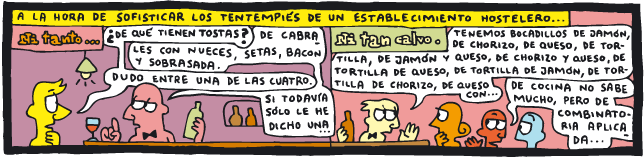
\includegraphics[width=1\textwidth]{imagenes/apendices/app11.png}
	\caption*{\scriptsize{Chiste de \textbf{Mario} en el diario \textbf{Público} publicado el 22/10/2008}\normalsize{.}}
	\end{figure}
\end{myexampleblock}


\chapter{Tablas distribución Binomial y Normal}

\begin{myexampleblock}{Chiste}
	\begin{figure}[H]
	\centering
	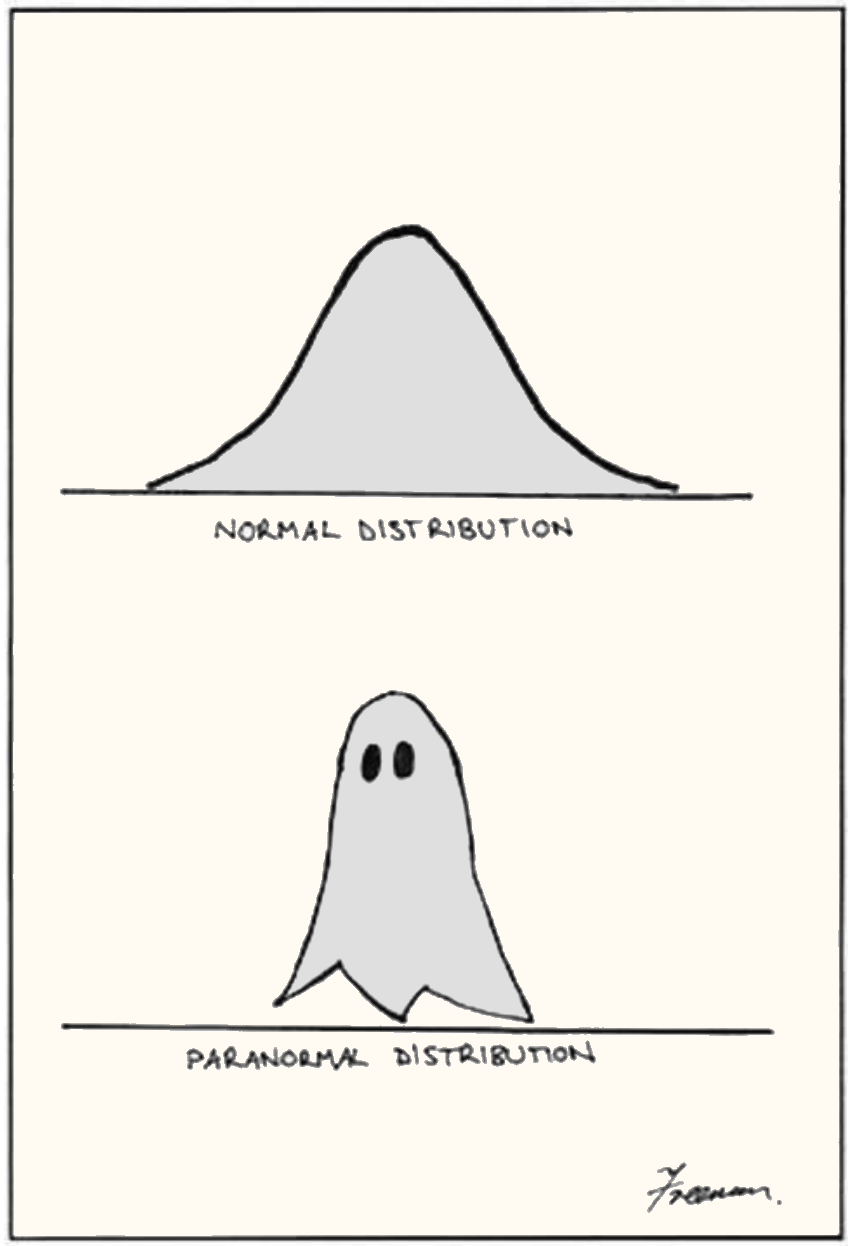
\includegraphics[width=.65\textwidth]{imagenes/apendices/app15.png}
	\end{figure}
\end{myexampleblock}


\newpage
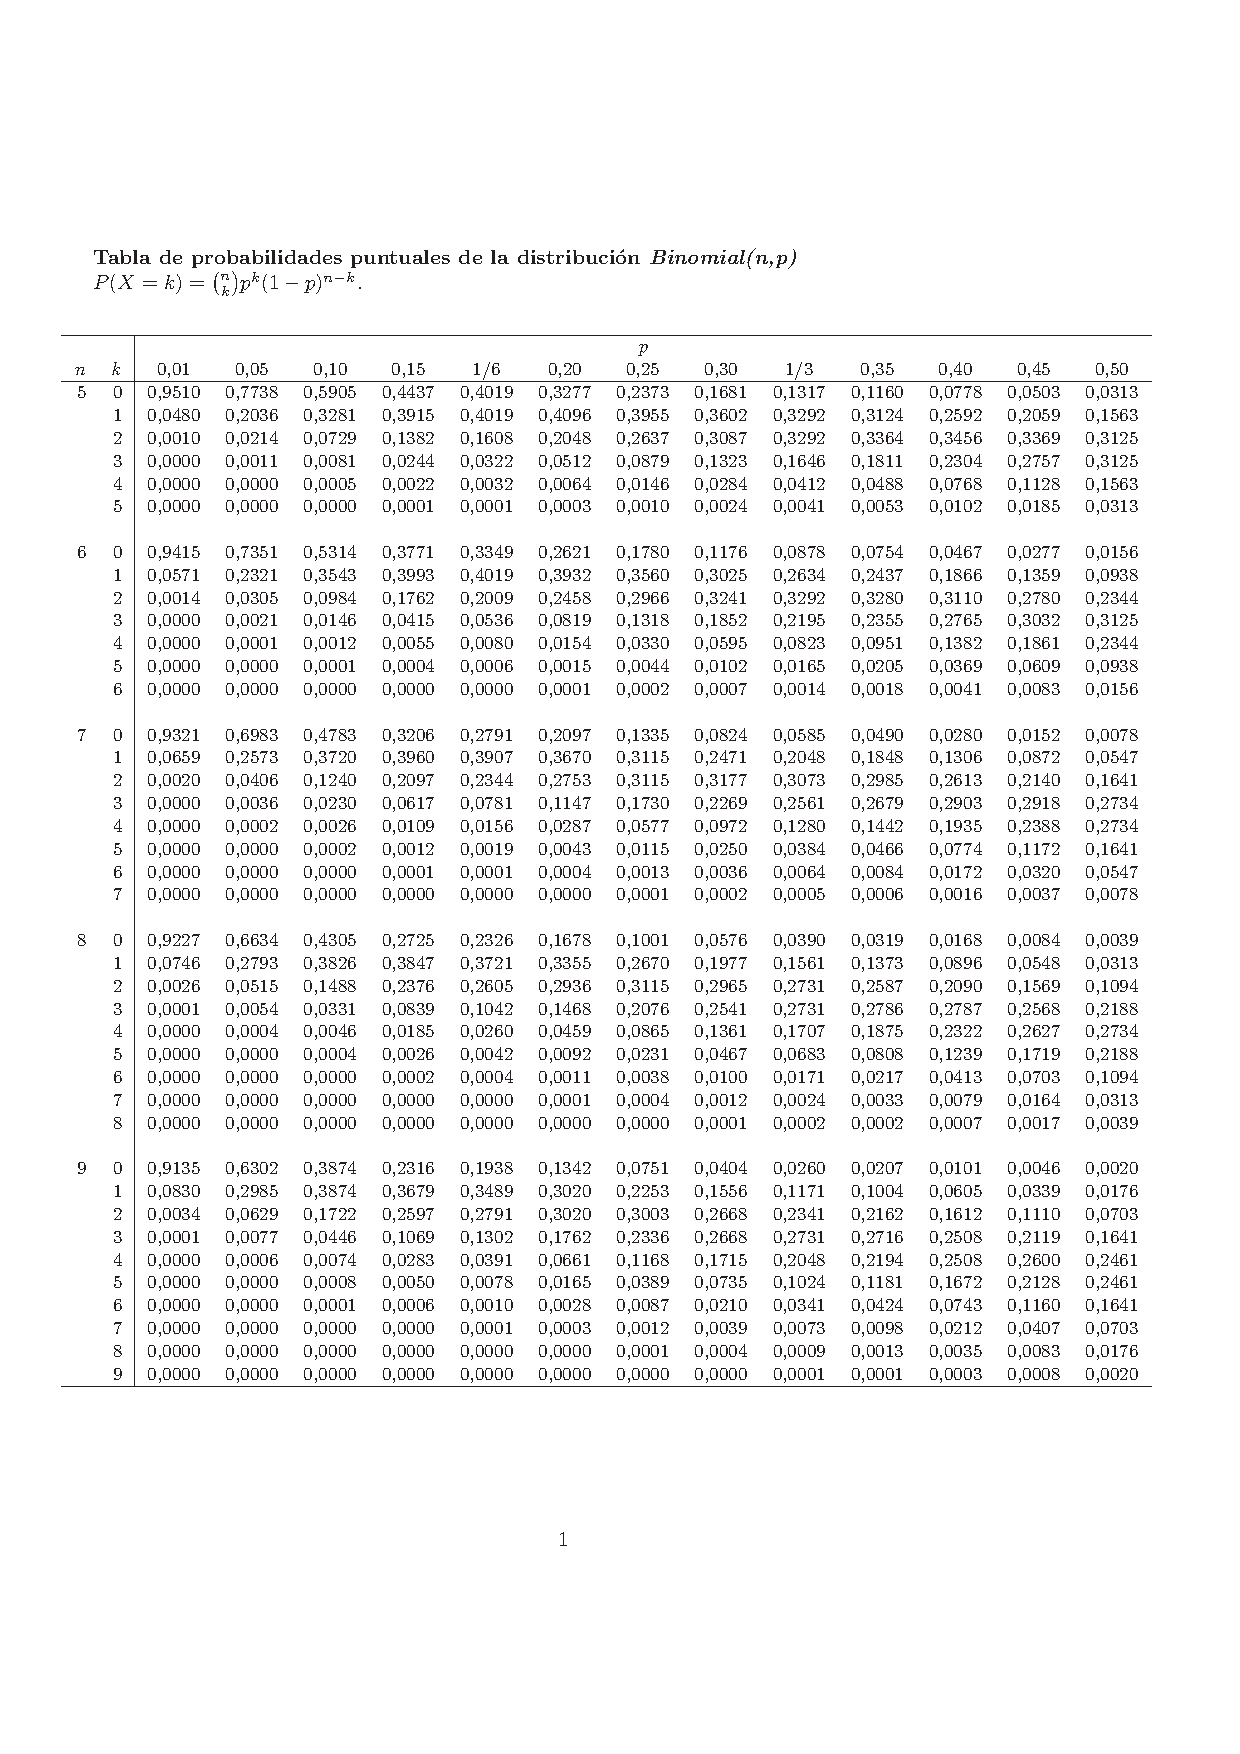
\includepdf[pages=-]{imagenes/apendices/tablas-distrib-prob.pdf}













\chapter{El problema del borracho $\divideontimes$} 



\section*{Enunciado}

\begin{ejemplo}
\textbf{Un borracho parte de un farol dando pasos de igual longitud hacia ambos lados. ?`Cuál es la probabilidad de que después de $N$ pasos vuelva al farol?}
\end{ejemplo}


\section{Esquema general de la resolución}

En la Sección \ref{sec:a} se analiza el problema desde una perspectiva general: se encuentra la probabilidad de que el borracho llegue, tras $N$ pasos, cada uno con probabilidad $p$ de avanzar hacia la derecha, a una posición $m$. Posteriormente, se hace $m = 0$ para dar respuesta a la pregunta del enunciado y se analizan los límites y el caso particular $p = \frac{1}{2}$, presentando gráficamente los principales resultados.


\begin{comment}
	Se deduce una equivalencia entre este problema y el problema anterior, lo que permite obtener, en general, la probabilidad de que los borrachos acaben separados $m$ posiciones tras dar $N$ pasos cada uno. Seguidamente se analiza el caso de $m = 0$, tanto analítica como gráficamente. Finalmente, se presenta un método alternativo de resolución de este mismo problema, para el caso particular $p = \frac{1}{2}$, basado en un resultado matemático conocido como \textit{identidad de Vandermonde}. Una demostración sencilla de la misma se ofrece en el Apéndice \ref{sec:vandermonde}
\end{comment}


\section{Resolución del problema}
\label{sec:a}
Sea un \textit{borracho unidimensional}, que queda representado matemáticamente por una única variable: su posición, $m \in \mathbb Z$. Se ha supuesto, sin pérdida de generalidad (pues corresponde a tomar, arbitrariamente, un origen), que el borracho parte de $m_0 = 0$. 

El borracho da $N$ pasos. Un \textit{paso} es un proceso en que se modifica la posición del borracho. Tras cada paso, la posición del borracho podrá, bien incrementarse en una unidad (lo que se denominará \textit{dar un paso a la derecha}), bien decrementarse en una unidad (\textit{dar un paso a la izquierda})\footnote{Se han tomado los pasos de igual longitud, tal y como indica el enunciado.}. Estos sucesos son obviamente \textit{mutuamente excluyentes} y \textit{complementarios} (en cada paso se da uno y sólo uno de ellos). Por tanto, si la probabilidad, en cada uno de los pasos, de que éste sea hacia la derecha es $p$, necesariamente la probabilidad de que el paso sea a la izquierda es $q \equiv 1 - p$, de modo que $p + q = 1$. Esto también implica que, si tras los $N$ pasos, $n_1$ han sido a la derecha, el número de pasos a la izquierda habrá sido $n_2 \equiv N - n_1$.

Con estas definiciones previas, se está ya en disposición de resolver el problema.

\subsection{Distribución binomial}
\label{sec:a_binomial}

El objetivo de esta sección es calcular la probabilidad, $W_N(n_1)$, de que, tras $N$ pasos, $n_1$ hayan sido hacia la derecha y los restantes, $N - n_1$, hacia la izquierda. 

Considérese, en primer lugar, la probabilidad de que se dé una secuencia concreta de pasos a izquierda y derecha, de modo que se cumpla la restricción anterior\footnote{Esto es, no se exige sólo que el número total de pasos a la derecha sea $n_1$, sino, además, que se den en un orden concreto.}. Como cada paso es un evento independiente, y $n$ eventos independientes, $\{S_i\}_{i=1}^n$, cumplen que 

\begin{equation}
	P \left(\bigcap\limits^n_{i=1} S_i \right) = \prod\limits^n_{i=1} P\left(S_i\right),
	\label{eq:eventos_independientes}
\end{equation}

\noindent entonces la probabilidad buscada, para una combinación como la descrita, no es más que $p^{n_1} (1-p)^{N-n_1}$, donde se han tenido en cuenta las ligaduras en $q$ y $n_2$. Sin embargo, no existe una única combinación de pasos a izquierda y derecha que resultan en $n_1$ pasos totales a derecha, sino que existen multitud de ellas.

Para cuantificarlas, es posible imaginar que existen tantas combinaciones posibles como maneras distintas hay de elegir $n_1$ elementos indistinguibles de un total de $N$. Esta cantidad no es más que\footnote{Deducir esto es relativamente sencillo. Dados $N$ elementos, de los que hay que elegir $n_1$, tenemos $N$ posibilidades para el primero, $N-1$ para el segundo, ..., y ($N-n_1+1$) para el $n_1$-ésimo. Cada elección es independiente y por tanto esto da $N(N-1)\cdots (N-n_1+1) \equiv \frac{N!}{(N-n_1)!}$ posibilidades distintas. Sin embargo, como los elementos son indistinguibles, es indiferente haber elegido los $n_1$ elementos en cualquier orden. Cada combinación única se ha tenido en cuenta $n_1!$ veces (el número de permutaciones de $n_1$ elementos). Por tanto, el número real de combinaciones de $N$ elementos de los que se escogen $n_1$ es $\frac{N!}{(N-n_1)! n_1!} \equiv \binom{N}{n_1} = \binom{N}{N-n_1}$, número al que se llama \textit{coeficiente binomial}.} el número combinatorio $\binom{N}{n_1}$. Por tanto, como todas las combinaciones son equiprobables, y se conoce la probabilidad de una de ellas y el número total de combinaciones que cumplen el requisito establecido, es directo afirmar que la probabilidad buscada es:

\begin{equation}
	W_N(n_1) = \binom{N}{n_1} p^{n_1} (1-p)^{N-n_1}
	\label{eq:distr_binomial}
\end{equation}

\subsection{Distribución en función de la posición final}
\label{sec:a_posicion}

Si la posición inicial es $m_0 = 0$, y se toma como criterio de signos positivo hacia la derecha, siendo los pasos de igual longitud, la posición tras los $N$ pasos será:

\begin{equation}
	m = n_1 - n_2 = n_1 - (N - n_1) = 2n_1 - N
	\label{eq:posicionfinal}
\end{equation}

Pueden comprobarse las siguientes propiedades intuitivas a partir de esta ecuación:

\begin{enumerate}
	\item Como $0 \leq n_1 \leq N$, entonces $- N \leq m \leq N$. En $N$ pasos, el borracho no puede alejarse más de $N$ posiciones de la inicial.
	\item Como $2n_1$ es par $\forall n_1 \in \mathbb N$, entonces $m$ y $N$ son ambos pares o impares. Con un número par de pasos, sólo es posible acceder a las posiciones pares como estado final. La afirmación análoga para los impares es igualmente cierta.
	\begin{enumerate}
		\item Como corolario a este resultado, para que $m = 0$, $N$ ha de ser par.
	\end{enumerate}
\end{enumerate}

Despejando de la ecuación \ref{eq:posicionfinal}, $n_1 = \frac{N+m}{2}$.  Sustituyendo esto último en la ecuación \ref{eq:distr_binomial}, y llamando $P\left(x = m | N\right)$ a la probabilidad de que la posición tras $N$ pasos sea $m$, se llega al resultado\footnote{También se ha calculado, con álgebra elemental, $N - n_1 = N - \frac{m+N}{2} = \frac{N-m}{2}$.}:

\begin{equation}
	P(x=m | N) = W_N\left(n_1 = \frac{m+N}{2}\right) = \frac{N!}{\left(\frac{N+m}{2} \right)! \left(\frac{N-m}{2} \right)!} \,p^{\frac{N+m}{2}} (1-p)^{\frac{N-m}{2}}
	\label{eq:prob_posfinal}
\end{equation}

Las propiedades 1 y 2 deducidas anteriormente garantizan que los números $\frac{N+m}{2}$, $\frac{N-m}{2} \in \mathbb N$, y por tanto los factoriales están bien definidos. Aunque no se pide explícitamente, puede ser interesante comprobar que, en el caso extremo, cuando $m = N$, el prefactor (i.e., el coeficiente binomial) toma como valor la unidad y, entonces, $P\left(x = N | N\right) = p^N$. Sólo existe una posibilidad: que todos los movimientos sean hacia la derecha. El análisis para $m = - N$ es del todo análogo, obteniéndose $(1-p)^N$ como resultado. Con $0 \leq p \leq 1$, $P(x = \pm N | N)$ definen sendas sucesiones monótonas y decrecientes, con límite 0 cuando $N \to \infty$. Esto indica que, \emph{a mayor número de pasos, la probabilidad de que el borracho llegue cualquiera de los extremos cae exponencialmente}.

\subsection{Probabilidad de volver al farol: caso particular $m = 0$}
\label{sec:a_volver}

La probabilidad de que el borracho vuelva a la posición inicial puede ser obtenida fácilmente, sin más que sustituir $m = 0$ en la ecuación \ref{eq:prob_posfinal}. Teniendo en cuenta, como se ha deducido previamente (propiedad 2.1 de la Sección \ref{sec:a_binomial}), que $N$ ha de ser par, se tiene la probabilidad dada por la ecuación \ref{eq:prob_volver}.

\begin{equation}
	\boxed{
	P(x=0 | N) = \frac{N!}{\left(\frac{N}{2} \right)! \left(\frac{N}{2} \right)!} \,p^{N/2} (1-p)^{N/2} = \binom{N}{\frac{N}{2}} \left[p(1-p)\right]^\frac{N}{2}
	}
	\label{eq:prob_volver}
\end{equation}

Es posible, previo a la representación gráfica, analizar ciertas propiedades del resultado obtenido.

\begin{itemize}
	\item Si se analiza la dependencia de la probabilidad obtenida con $p$, al ser $P(x=0|N)$ una función monótona y creciente de $p(1-p)$, los máximos de $P$ se corresponden con los máximos de $p(1-p)$. Esta última es una parábola invertida con vértice en $p = \frac{1}{2}$, por lo que se puede concluir que \emph{la probabilidad de que el borracho vuelva a la posición inicial se maximiza cuando ambos pasos, a izquierda y derecha, son igualmente probables}. Resulta razonable que, de no ser así, existirá un sesgo que favorecerá que la posición final sea aquella cuyos pasos son más probables\footnote{De hecho, el valor esperado de $n_1$ vendrá dado, según la expresión del valor esperado de una variable binomial, por $\bar {n_1} = Np$. Utilizando la ecuación \ref{eq:posicionfinal}, $\bar{m} = N (2p-1)$.}.
	\item El factor $\binom{N}{\frac{N}{2}}$, que da el número de combinaciones posibles que devuelven al borracho a la posición inicial, crece\footnote{Esto puede deducirse de la identificación de los coeficientes binomiales con los valores del \textit{triángulo de Pascal} o \textit{triángulo de Tartaglia}. Este coeficiente binomial recibe el nombre de \textit{coeficiente binomial central}, y se corresponde con los valores sobre el eje de simetría del triángulo. Estos valores crecen con $N$, lo que demuestra la afirmación precedente.} con el número, $N$, de pasos. Por otro lado, al ser $p(1-p) < 1$, el factor $[p(1-p)]^{\frac{N}{2}}$ cae con $N$: cada una de las posibles combinaciones es menos probable. Por tanto, parece complicado deducir si $P(x=0|N)$ crecerá o decrecerá con $N$. Por ello, se dará respuesta a este interrogante a partir de la representación gráfica, o bien, a partir del análisis de un caso particular.
\end{itemize}

\subsubsection{Caso particular: ambos sucesos equiprobables ($p = \frac{1}{2}$)}
\label{sec:a_volver_1/2}
En el caso partícular $p = \frac{1}{2}$, esto es, el borracho tiene igual probabilidad de moverse a izquierda o derecha en cada paso, la ecuación \ref{eq:prob_volver} se simplifica a:

\begin{equation}
	P_{p = \frac{1}{2}}(x=0|N)=\binom{N}{\frac{N}{2}}\frac{1}{2^N}
	\label{eq:prob_volver_1/2}
\end{equation}

Esta expresión, además de ser más simple, permite analizar el caso límite $N\to \infty$. Si se tiene en cuenta que $\binom{N}{\frac{N}{2}}$ es el coeficiente binomial central, el elemento central de la fila $N$ del triángulo de Pascal (donde $N$ es par), y que $2^N$ es la suma de los elementos de la $N$-ésima fila, la probabilidad obtenida no es más que la razón entre estos dos números. Esta razón disminuye\footnote{Aunque no se demuestra explícitamente este resultado, porque excede el objetivo de este análisis, puede ``comprobarse'': para la fila $N=2$, dicho cociente es $\frac{2}{2^2} = 0.5$; para la fila $N=4$, $\frac{6}{2^4} = 0.375$; para la fila $N = 16$, $\frac{12870}{2^16} \approx 0.196$.} con $N\to \infty$. Según habíamos analizado, $p=\frac{1}{2}$ daba la máxima probabilidad a un $N$ fijo. Por tanto, es una cota superior de la probabilidad de que el borracho vuelva al origen, para cada $N$. 

Como la cota superior decrece con $N$, este razonamiento permite concluir que, \emph{a mayor número de pasos $N$, menor es la probabilidad de que el borracho vuelva al origen}.

\subsection{Análisis gráfico de las ecuaciones \ref{eq:prob_posfinal} y \ref{eq:prob_volver}}
\label{sec:a_grafico}

En primer lugar, se pretende observar gráficamente cómo se distribuye la probabilidad de que el borracho acabe, tras $N$ pasos, en una posición final $m$. En este análisis, se han fijado $N$ y $p$, y se ha graficado la ecuación \ref{eq:prob_posfinal} en función de $m$. La propiedad 2 de la Sección \ref{sec:a_posicion} establece que $m$ y $N$ son ambos pares o impares. Se han tomado $N$ pares para ejemplificar. La probabilidad de que el borracho acabe en $m$ impares es, por tanto, nula. Para la claridad de la representación gráfica, se han representado los puntos de $m$ par, y se han unido los resultados con líneas. En todo caso, ha de tenerse en cuenta que la distribución es discreta y sólo está definida para $m\in\mathbb N$, aunque se hayan introducido las líneas para facilitar la visualización.

\begin{figure}[h!]
	\centering
	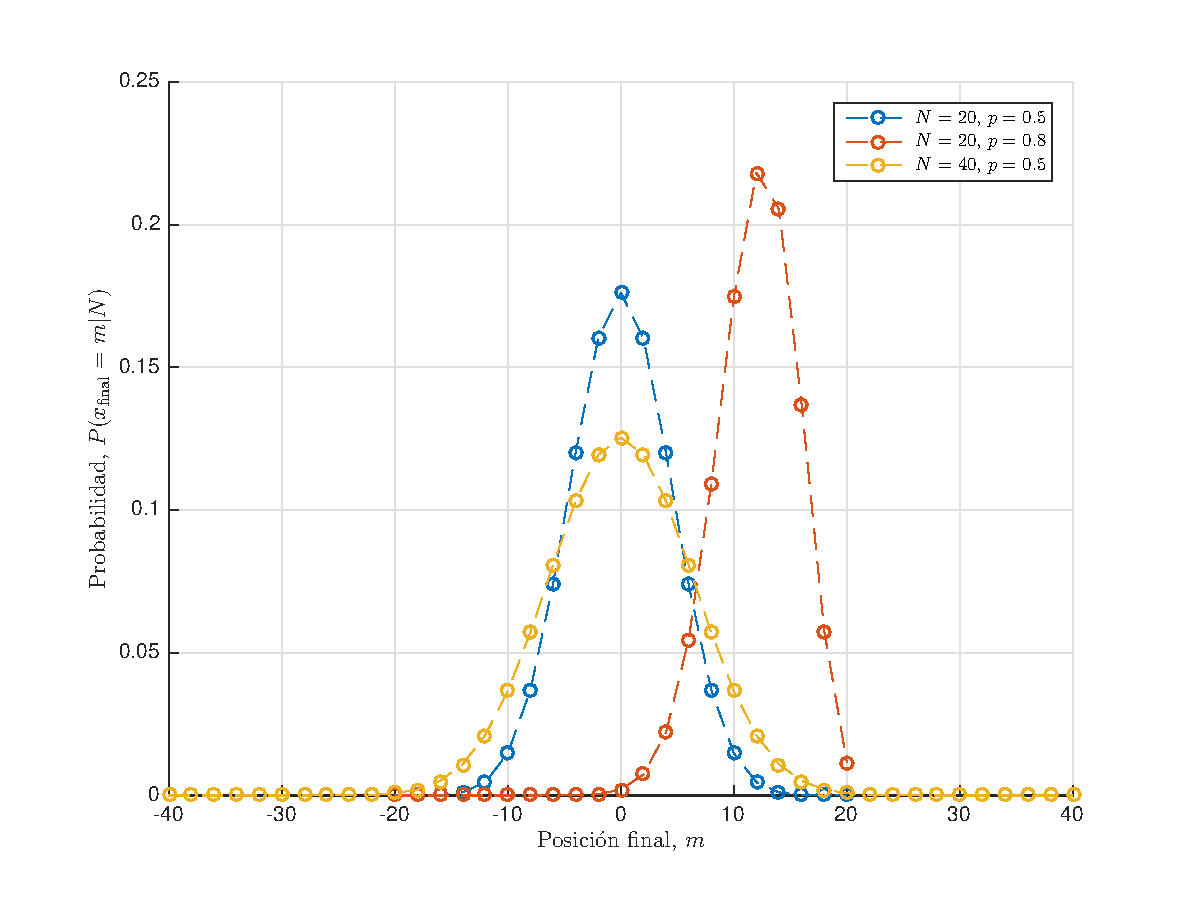
\includegraphics[width = 0.8\linewidth]{prob_posfinal}
	\vspace{-0.5cm}
	\caption{\small Probabilidad de que el borracho, tras $N$ pasos, acabe en una posición $m$. Se han estudiado varios casos, variando tanto $p$ como $N$, que se encuentran detallados en la leyenda.}
	\label{fig:prob_posfinal}
\end{figure}

En la Figura \ref{fig:prob_posfinal} se muestran diversas distribuciones de probabilidad de que el borracho acabe en una posición $m$.

\begin{itemize}
	\item La curva azul ha sido generada con $N = 20$ y pasos a cada lado igualmente probables, $p=0.5$. Tal y como sería razonable, en estas condiciones la distribución de probabilidad es par ($P(m) =P(-m)$) y tiene máximo en $m=0$: la posición final más probable es el origen. Sin embargo, los valores de $m$ cercanos a 0 tienen también probabilidades elevadas, y los valores extremos de $m$ (cercanos a $\pm N$) son altamente improbables (corresponden a [casi] todos los pasos del borracho en un mismo sentido).
	\item Manteniendo fijo el número de pasos, $N=20$, se ha variado la probabilidad $p$ de que el paso sea hacia la derecha, haciendo este suceso más probable ($p>0.5$). Consecuentemente, toda la gráfica se ha distorsionado, desplazándose hacia la derecha. Con $p=0.8$, el valor esperado de los pasos a derecha, $n_1$, es $Np = 16$. Así, 4 pasos son hacia la izquierda y el valor esperado de $m$ sería 12, lo que concuerda a la perfección con la línea roja de la gráfica.
	\item Con $p=0.5$ pero duplicando $N$, se obtiene, de nuevo, una curva con simetría par. Sin embargo, ésta se ha suavizado (presenta un pico menor): aunque el valor más probable sigue siendo $m=0$, éste es ahora menos probable. Esto está en concordancia con lo deducido en la Sección \ref{sec:a_volver_1/2}: la probabilidad de volver al origen cae a medida que $N$ toma valores mayores. Al mismo tiempo, la distribución ha crecido en anchura (ahora son posibles valores más lejanos de $m$), pero no en anchura relativa (pese a que $N$ se ha duplicado, la anchura de la distribución ha crecido en un factor menor).
\end{itemize}

\begin{figure}[h!]
	\centering
	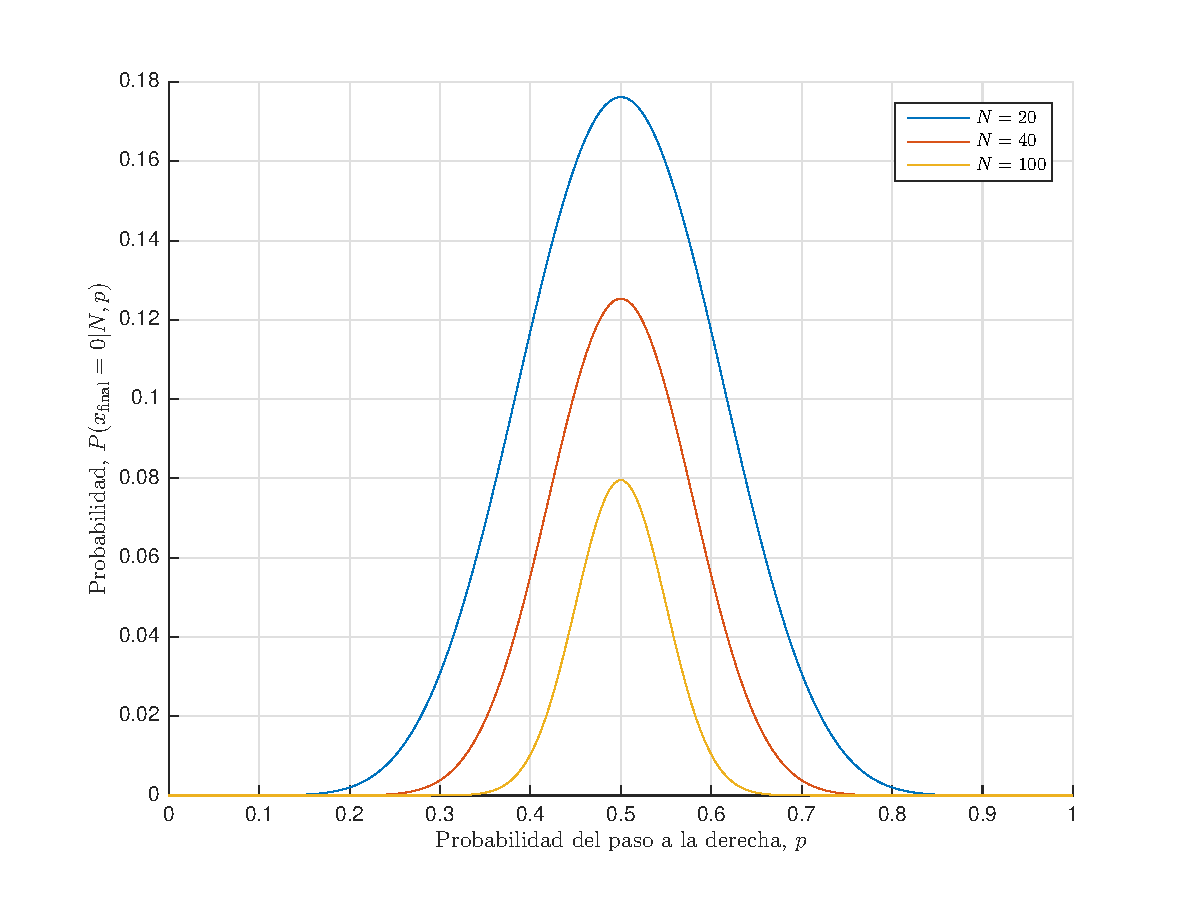
\includegraphics[width = 0.8\linewidth]{prob_volver}
	\vspace{-0.5cm}
	\caption{\small Probabilidad de que el borracho, tras $N$ pasos y con probabilidad $p$ de que cada paso sea a la derecha, vuelva a la posición inicial.}
	\label{fig:prob_volver}
\end{figure}

Por otro lado, se ha analizado la ecuación \ref{eq:prob_volver} manteniendo $N$ constante en función de $p$ (que puede tomar cualquier valor real entre 0 y 1). Para varios $N$, se muestran las curvas de probabilidad de que el borracho vuelva a la posición inicial en función de $p$ en la Figura \ref{fig:prob_volver}.

Se observa, tal y como se había apuntado, que la máxima probabilidad de que el borracho vuelva se da cuando $p = \frac{1}{2}$ (entonces, el valor esperado de pasos a izquierda y derecha coinciden); y que, a mayores $N$, cae la probabilidad de que el borracho regrese al origen (no obstante, sigue siendo, en todo caso, el resultado más probable $\forall N$). Además, es también interesante señalar que, a medida que $N$ se incrementa, la anchura de la distribución de probabilidad en función de $p$ decrece: es decir, a mayores $N$, la ventana de valores de $p$ que permiten que la probabilidad de regreso del borracho a su posición inicial tenga valores no despreciables se hace más pequeña. Esto es razonable, ya que, cuando $N$ aumenta, la dispersión de valores en torno al valor esperado también aumenta (ver Figura \ref{fig:prob_posfinal}), y es necesario restringirse a $p$ más cercanos a $\frac{1}{2}$ para que la probabilidad de que el borracho vuelva al origen sea alta.

\rule{300pt}{0.1pt}

\begin{flushright}
	Problema resuelto por \emph{David Vallés Pérez.}
\end{flushright}


